% Seminar 9: ARCH and GARCH models
% Statistics of Financial Markets -- Bachelor's programme, Bucharest University of Economic Studies
% GENERATED by latex/build_seminar9.py -- edit the generator, not this file.
% Student version by default; the instructor version is the *_solutions.tex wrapper.
\makeatletter\@ifundefined{ifsolutions}{\expandafter\newif\csname ifsolutions\endcsname}{}\makeatother

\newcommand{\coursename}{Statistics of Financial Markets}
% Preambul comun SFM -- Statistica piețelor financiare / Statistics of Financial Markets (Beamer, 16:9)
% Același design ca MFM. Înainte de % Preambul comun SFM -- Statistica piețelor financiare / Statistics of Financial Markets (Beamer, 16:9)
% Același design ca MFM. Înainte de % Preambul comun SFM -- Statistica piețelor financiare / Statistics of Financial Markets (Beamer, 16:9)
% Același design ca MFM. Înainte de \input{../../latex/preamble} se definește
%   \newcommand{\coursename}{Statistics of Financial Markets}      (EN)
%   \newcommand{\coursename}{Statistica piețelor financiare}       (RO)  și  \def\sfmlang{ro}
% Fișierele .tex se află în EN/Courses, EN/Seminars, RO/Cursuri, RO/Seminarii (două niveluri sub rădăcină).
% Deck-urile sînt generate de latex/build_chapterN.py / build_seminarN.py (vezi latex/sfm_build.py).

\documentclass[9pt, aspectratio=169, t]{beamer}
\providecommand{\coursename}{Statistics of Financial Markets}

% Ensure content fits on slides
\setbeamersize{text margin left=8mm, text margin right=8mm}

%=============================================================================
% THEME AND STYLE CONFIGURATION
%=============================================================================
\usetheme{default}
% Using default theme for clean header/footer control

% Color Palette (matching Redispatch PDF)
\definecolor{MainBlue}{RGB}{26, 58, 110}
\definecolor{AccentBlue}{RGB}{26, 58, 110}
\definecolor{IDAred}{RGB}{205, 0, 0}
\definecolor{DarkGray}{RGB}{51, 51, 51}
\definecolor{MediumGray}{RGB}{128, 128, 128}
\definecolor{LightGray}{RGB}{248, 248, 248}
\definecolor{VeryLightGray}{RGB}{235, 235, 235}
\definecolor{KeynoteGray}{RGB}{218, 218, 218}
\definecolor{SectionGray}{RGB}{120, 120, 120}
\definecolor{FooterGray}{RGB}{100, 100, 100}
\definecolor{Crimson}{RGB}{220, 53, 69}
\definecolor{Forest}{RGB}{46, 125, 50}
\definecolor{Amber}{RGB}{181, 133, 63}
\definecolor{Orange}{RGB}{230, 126, 34}
\definecolor{Purple}{RGB}{142, 68, 173}

% Gradient background (exact Keynote 315° gradient: white to RGB 218,218,218)
\setbeamertemplate{background}{%
    \begin{tikzpicture}[remember picture, overlay]
        \shade[shading=axis, shading angle=315,
        top color=white, bottom color=KeynoteGray]
        (current page.south west) rectangle (current page.north east);
    \end{tikzpicture}%
}
% Fallback solid color for compatibility
\setbeamercolor{background canvas}{bg=}

\setbeamercolor{palette primary}{bg=MainBlue, fg=white}
\setbeamercolor{palette secondary}{bg=MainBlue!85, fg=white}
\setbeamercolor{palette tertiary}{bg=MainBlue!70, fg=white}
\setbeamercolor{structure}{fg=MainBlue}
\setbeamercolor{title}{fg=IDAred}
\setbeamercolor{frametitle}{fg=IDAred, bg=}
\setbeamercolor{block title}{bg=MainBlue, fg=white}
\setbeamercolor{block body}{bg=VeryLightGray, fg=DarkGray}
\setbeamercolor{block title alerted}{bg=Crimson, fg=white}
\setbeamercolor{block body alerted}{bg=Crimson!8, fg=DarkGray}
\setbeamercolor{block title example}{bg=Forest, fg=white}
\setbeamercolor{block body example}{bg=Forest!8, fg=DarkGray}
\setbeamercolor{item}{fg=MainBlue}

% Footer colors (override Madrid theme blue)
\setbeamercolor{author in head/foot}{fg=FooterGray, bg=}
\setbeamercolor{title in head/foot}{fg=FooterGray, bg=}
\setbeamercolor{date in head/foot}{fg=FooterGray, bg=}
\setbeamercolor{section in head/foot}{fg=FooterGray, bg=}
\setbeamercolor{subsection in head/foot}{fg=FooterGray, bg=}

% Bullet styles (apply everywhere including blocks)
\setbeamertemplate{itemize item}{\color{MainBlue}$\boxdot$}
\setbeamertemplate{itemize subitem}{\color{MainBlue}$\blacktriangleright$}
\setbeamertemplate{itemize subsubitem}{\color{MainBlue}\tiny$\bullet$}
\setbeamertemplate{itemize/enumerate body begin}{\normalsize}
\setbeamertemplate{itemize/enumerate subbody begin}{\normalsize}

% Item spacing - compact style
\setlength{\leftmargini}{10pt}       % Level 1: minimal indent
\setlength{\leftmarginii}{10pt}      % Level 2: minimal additional indent
% Compact list spacing (zero extra space before/after lists in blocks)
\makeatletter
\def\@listi{\leftmargin\leftmargini \topsep 0pt \parsep 0pt \itemsep 0pt}
\def\@listii{\leftmargin\leftmarginii \topsep 0pt \parsep 0pt \itemsep 0pt}
\makeatother

\setbeamertemplate{navigation symbols}{}

%=============================================================================
% CUSTOM HEADLINE
%=============================================================================
\setbeamertemplate{headline}{%
    \vskip10pt%
    \hbox to \paperwidth{%
        \hskip0.5cm%
        {\small\color{FooterGray}\renewcommand{\hyperlink}[2]{##2}\insertsectionhead}%
        \hfill%
        \textcolor{FooterGray}{\small\insertframenumber}%
        \hskip0.5cm%
    }%
    \vskip4pt%
    {\color{FooterGray}\hrule height 0.4pt}%
}

%=============================================================================
% CUSTOM FOOTER
%=============================================================================
\usepackage{fontawesome5}

\setbeamertemplate{footline}{%
    {\color{FooterGray}\hrule height 0.4pt}%
    \vskip4pt%
    \hbox to \paperwidth{%
        \hskip0.5cm%
        \textcolor{FooterGray}{\small\coursename}%
        \hfill%
        \raisebox{-0.1em}{%
            \begin{tikzpicture}[x=0.08em, y=0.08em, line width=0.4pt]
                \draw[FooterGray] (0,3) -- (1,4) -- (2,3.5) -- (3,5) -- (4,4) -- (5,6) -- (6,5.5) -- (7,4) -- (8,5) -- (9,7) -- (10,6) -- (11,5) -- (12,6.5) -- (13,8) -- (14,7) -- (15,6) -- (16,7.5) -- (17,9) -- (18,8) -- (19,7) -- (20,8.5) -- (21,10) -- (22,9) -- (23,8) -- (24,9.5);
            \end{tikzpicture}%
        }%
        \hskip0.5cm%
    }%
    \vskip6pt%
}

%=============================================================================
% PACKAGES
%=============================================================================
\usepackage[utf8]{inputenc}
\DeclareUnicodeCharacter{03B1}{\ensuremath{\alpha}}
\usepackage[T1]{fontenc}
\usepackage{amsmath, amssymb, amsthm}
\usepackage{mathtools}
\usepackage{bm}
\usepackage{tikz}
\usetikzlibrary{arrows.meta, positioning, shapes, calc, decorations.pathreplacing, shadings}
\usepackage{booktabs}
\usepackage{multirow}
\usepackage{array}
\usepackage{graphicx}
\usepackage{hyperref}
\usepackage{colortbl}
\usepackage{listings}
\lstset{language=Python, basicstyle=\ttfamily\scriptsize, keywordstyle=\color{MainBlue}\bfseries,
  commentstyle=\color{Forest}, stringstyle=\color{Crimson}, breaklines=true,
  frame=none, backgroundcolor=\color{VeryLightGray}, xleftmargin=2mm}
\hypersetup{colorlinks=true, linkcolor=MainBlue, urlcolor=MainBlue}
\graphicspath{{../../logos/}{../../charts/}{../../photos/}}
\usepackage{xcolor}
\hfuzz=2pt  % Suppress tiny overfull warnings (<2pt)
\vfuzz=2pt  % Suppress tiny vertical overfull warnings (<2pt)

%=============================================================================
% QUANTLET COMMANDS
%   \quantlet{<displayed name>}{<url>}       (generic, compatible with the older SFM decks)
%   \sfmquantlet{Ch_05}{SFM_ch5_garch}       -> https://github.com/danpele/SFM/tree/main/Quantlets/Ch_05/SFM_ch5_garch
%   \qlurl{<folder>} is defined per chapter by the generator (Quantlets/Ch_NN/<folder>)
%=============================================================================
\newcommand{\sfmrepo}{https://github.com/danpele/SFM}
\newcommand{\sfmqlbase}{https://github.com/danpele/SFM/tree/main/Quantlets}
\newcommand{\quantlet}[2]{%
    \hfill\href{#2}{%
        \raisebox{-0.15em}{
\includegraphics[height=0.7em]{ql_logo.png}}%
        \textcolor{MainBlue}{\tiny\ #1}%
    }%
}
\newcommand{\sfmquantlet}[2]{\quantlet{\detokenize{#2}}{\sfmqlbase/#1/#2}}

%=============================================================================
% NOTEBOOKS (Google Colab)
%   \colaburl{notebooks/EN/chapter5_seminar_notebook.ipynb} -> the Colab link of a file in the SFM repo
%   \nb: the chapter notebook (each seminar deck redefines it with \renewcommand)
%=============================================================================
\newcommand{\colaburl}[1]{https://colab.research.google.com/github/danpele/SFM/blob/main/#1}
\newcommand{\nb}{https://colab.research.google.com/github/danpele/SFM/tree/main/notebooks/EN}
\newcommand{\nbname}{notebooks/EN}

%=============================================================================
% SLIDE HELPERS (used by the generators; the same as in MFM)
%=============================================================================
% local font size for list bodies (the preamble forces \normalsize)
\newcommand{\itemsize}[1]{\setbeamertemplate{itemize/enumerate body begin}{#1}\setbeamertemplate{itemize/enumerate subbody begin}{#1}}
\newcommand{\intitle}[1]{{\hypersetup{urlcolor=white}#1}}   % white links inside coloured title bars
\newcommand{\imgcap}[1]{{\scriptsize #1}\\[0.5mm]}          % caption under a photo
\newcommand{\imgcredit}[2]{{\tiny\color{FooterGray}\href{#1}{#2}}}   % image credit: source URL, author/licence
\newcommand{\aiprompt}[1]{{\ttfamily\color{MainBlue}#1}}     % a prompt to an AI assistant

%=============================================================================
% SEMINARS: student version by default; the instructor wrapper *_solutions.tex sets \solutionstrue
%=============================================================================
\makeatletter\@ifundefined{ifsolutions}{\expandafter\newif\csname ifsolutions\endcsname}{}\makeatother
\newcommand{\solonly}[1]{\ifsolutions #1\fi}
\newcommand{\propsub}{\ifsolutions\else\framesubtitle{\ifdefined\sfmlang Rezolvarea se discută la seminar\else Solution discussed in class\fi}\fi}

%=============================================================================
% APPENDIX AND CHAPTER LINKS (latex/appendix_links.py writes the calls; it also re-declares these
% macros before \begin{document}, so the decks compile with or without this preamble block)
%=============================================================================
\providecommand{\sfmapplink}[3]{\hypertarget{#2}{}\hyperlink{#1}{\beamergotobutton{#3}}}
\providecommand{\sfmappback}[2]{\begin{tikzpicture}[remember picture,overlay]\node[anchor=south east] at ([xshift=-3mm,yshift=7mm]current page.south east){\hyperlink{#1}{\beamerreturnbutton{#2}}};\end{tikzpicture}}
\providecommand{\sfmchlink}[2]{\href{#1}{#2}}
\providecommand{\sfmchlinkt}[2]{\href{#1}{\usebeamercolor[fg]{frametitle}#2}}

%=============================================================================
% QUANTINAR COMMAND: link către un curs Quantinar (subiecte avansate)
%=============================================================================
\newcommand{\quantinar}[2]{%
    \href{#2}{%
        \raisebox{-0.15em}{
\includegraphics[height=0.8em]{qr_logo.png}}%
        \textcolor{MainBlue}{\scriptsize\ #1}%
    }%
}

%=============================================================================
% CUSTOM TITLE PAGE
%=============================================================================
\defbeamertemplate*{title page}{hybrid}[1][]
{
    \vspace{0.2cm}
    % Logos row - top header (with clickable links)
    \begin{center}
        \href{https://www.ase.ro}{
\includegraphics[height=1.0cm]{ase_logo.png}}\hspace{0.3cm}%
        \href{https://theida.net}{
\includegraphics[height=1.0cm]{ida_logo.png}}\hspace{0.3cm}%
        \href{https://blockchain-research-center.com}{
\includegraphics[height=1.0cm]{brc_logo.png}}\hspace{0.3cm}%
        \href{https://www.ai4efin.ase.ro}{
\includegraphics[height=1.0cm]{ai4efin_logo.png}}\hspace{0.3cm}%
        \href{https://ipe.ro/new}{
\includegraphics[height=1.0cm]{acad_logo.png}}\hspace{0.3cm}%
        \href{https://www.digital-finance-msca.com}{
\includegraphics[height=1.0cm]{msca_logo.png}}%
    \end{center}

    \vspace{0.6cm}

    % Main title with Q logos on sides (with clickable links)
    \begin{center}
        \begin{minipage}{0.1\textwidth}
            \centering
            \href{https://quantlet.com}{
\includegraphics[height=1.1cm]{ql_logo.png}}
        \end{minipage}%
        \begin{minipage}{0.78\textwidth}
            \centering
            {\LARGE\bfseries\usebeamercolor[fg]{title}\inserttitle}

            \vspace{0.3cm}

            {\usebeamerfont{subtitle}\usebeamercolor[fg]{title}\insertsubtitle}
        \end{minipage}%
        \begin{minipage}{0.1\textwidth}
            \centering
            \href{https://quantinar.com}{
\includegraphics[height=1.1cm]{qr_logo.png}}
        \end{minipage}
    \end{center}

    \vspace{0.6cm}

    % Authors (left aligned)
    \hspace{0.5cm}{\usebeamerfont{author}\insertauthor}

    \vspace{0.3cm}

    % Institute/Affiliations (left aligned)
    \hspace{0.5cm}\begin{minipage}[t]{0.9\textwidth}
        \raggedright\small\insertinstitute
    \end{minipage}
}

%=============================================================================
% THEOREM ENVIRONMENTS
%=============================================================================
\theoremstyle{definition}
\setbeamertemplate{theorems}[numbered]
\ifdefined\sfmlang
\newtheorem{defn}{Definiție}
\newtheorem{thm}{Teoremă}
\newtheorem{prop}{Propoziție}
\newtheorem{rmk}{Observație}
\else
\newtheorem{defn}{Definition}
\newtheorem{thm}{Theorem}
\newtheorem{prop}{Proposition}
\newtheorem{rmk}{Remark}
\fi

%=============================================================================
% CENTRED MINIPAGE (no extra vertical space)
%=============================================================================
\newenvironment{cminipage}[1]{%
    \par\noindent\hfill\begin{minipage}{#1}\ignorespaces
}{%
    \end{minipage}\hfill\null\par
}

%=============================================================================
% CUSTOM COMMANDS
%=============================================================================
\newcommand{\E}{\mathbb{E}}
\newcommand{\Var}{\text{Var}}
\newcommand{\Cov}{\text{Cov}}
\newcommand{\Corr}{\text{Corr}}
\newcommand{\R}{\mathbb{R}}
\newcommand{\N}{\mathbb{N}}
\newcommand{\Z}{\mathbb{Z}}
\newcommand{\B}{\mathbf{B}}
\newcommand{\imark}{\textcolor{MainBlue}{\textbullet}}
\newcommand{\RMSE}{\text{RMSE}}
\newcommand{\MAE}{\text{MAE}}
\newcommand{\MAPE}{\text{MAPE}}

 se definește
%   \newcommand{\coursename}{Statistics of Financial Markets}      (EN)
%   \newcommand{\coursename}{Statistica piețelor financiare}       (RO)  și  \def\sfmlang{ro}
% Fișierele .tex se află în EN/Courses, EN/Seminars, RO/Cursuri, RO/Seminarii (două niveluri sub rădăcină).
% Deck-urile sînt generate de latex/build_chapterN.py / build_seminarN.py (vezi latex/sfm_build.py).

\documentclass[9pt, aspectratio=169, t]{beamer}
\providecommand{\coursename}{Statistics of Financial Markets}

% Ensure content fits on slides
\setbeamersize{text margin left=8mm, text margin right=8mm}

%=============================================================================
% THEME AND STYLE CONFIGURATION
%=============================================================================
\usetheme{default}
% Using default theme for clean header/footer control

% Color Palette (matching Redispatch PDF)
\definecolor{MainBlue}{RGB}{26, 58, 110}
\definecolor{AccentBlue}{RGB}{26, 58, 110}
\definecolor{IDAred}{RGB}{205, 0, 0}
\definecolor{DarkGray}{RGB}{51, 51, 51}
\definecolor{MediumGray}{RGB}{128, 128, 128}
\definecolor{LightGray}{RGB}{248, 248, 248}
\definecolor{VeryLightGray}{RGB}{235, 235, 235}
\definecolor{KeynoteGray}{RGB}{218, 218, 218}
\definecolor{SectionGray}{RGB}{120, 120, 120}
\definecolor{FooterGray}{RGB}{100, 100, 100}
\definecolor{Crimson}{RGB}{220, 53, 69}
\definecolor{Forest}{RGB}{46, 125, 50}
\definecolor{Amber}{RGB}{181, 133, 63}
\definecolor{Orange}{RGB}{230, 126, 34}
\definecolor{Purple}{RGB}{142, 68, 173}

% Gradient background (exact Keynote 315° gradient: white to RGB 218,218,218)
\setbeamertemplate{background}{%
    \begin{tikzpicture}[remember picture, overlay]
        \shade[shading=axis, shading angle=315,
        top color=white, bottom color=KeynoteGray]
        (current page.south west) rectangle (current page.north east);
    \end{tikzpicture}%
}
% Fallback solid color for compatibility
\setbeamercolor{background canvas}{bg=}

\setbeamercolor{palette primary}{bg=MainBlue, fg=white}
\setbeamercolor{palette secondary}{bg=MainBlue!85, fg=white}
\setbeamercolor{palette tertiary}{bg=MainBlue!70, fg=white}
\setbeamercolor{structure}{fg=MainBlue}
\setbeamercolor{title}{fg=IDAred}
\setbeamercolor{frametitle}{fg=IDAred, bg=}
\setbeamercolor{block title}{bg=MainBlue, fg=white}
\setbeamercolor{block body}{bg=VeryLightGray, fg=DarkGray}
\setbeamercolor{block title alerted}{bg=Crimson, fg=white}
\setbeamercolor{block body alerted}{bg=Crimson!8, fg=DarkGray}
\setbeamercolor{block title example}{bg=Forest, fg=white}
\setbeamercolor{block body example}{bg=Forest!8, fg=DarkGray}
\setbeamercolor{item}{fg=MainBlue}

% Footer colors (override Madrid theme blue)
\setbeamercolor{author in head/foot}{fg=FooterGray, bg=}
\setbeamercolor{title in head/foot}{fg=FooterGray, bg=}
\setbeamercolor{date in head/foot}{fg=FooterGray, bg=}
\setbeamercolor{section in head/foot}{fg=FooterGray, bg=}
\setbeamercolor{subsection in head/foot}{fg=FooterGray, bg=}

% Bullet styles (apply everywhere including blocks)
\setbeamertemplate{itemize item}{\color{MainBlue}$\boxdot$}
\setbeamertemplate{itemize subitem}{\color{MainBlue}$\blacktriangleright$}
\setbeamertemplate{itemize subsubitem}{\color{MainBlue}\tiny$\bullet$}
\setbeamertemplate{itemize/enumerate body begin}{\normalsize}
\setbeamertemplate{itemize/enumerate subbody begin}{\normalsize}

% Item spacing - compact style
\setlength{\leftmargini}{10pt}       % Level 1: minimal indent
\setlength{\leftmarginii}{10pt}      % Level 2: minimal additional indent
% Compact list spacing (zero extra space before/after lists in blocks)
\makeatletter
\def\@listi{\leftmargin\leftmargini \topsep 0pt \parsep 0pt \itemsep 0pt}
\def\@listii{\leftmargin\leftmarginii \topsep 0pt \parsep 0pt \itemsep 0pt}
\makeatother

\setbeamertemplate{navigation symbols}{}

%=============================================================================
% CUSTOM HEADLINE
%=============================================================================
\setbeamertemplate{headline}{%
    \vskip10pt%
    \hbox to \paperwidth{%
        \hskip0.5cm%
        {\small\color{FooterGray}\renewcommand{\hyperlink}[2]{##2}\insertsectionhead}%
        \hfill%
        \textcolor{FooterGray}{\small\insertframenumber}%
        \hskip0.5cm%
    }%
    \vskip4pt%
    {\color{FooterGray}\hrule height 0.4pt}%
}

%=============================================================================
% CUSTOM FOOTER
%=============================================================================
\usepackage{fontawesome5}

\setbeamertemplate{footline}{%
    {\color{FooterGray}\hrule height 0.4pt}%
    \vskip4pt%
    \hbox to \paperwidth{%
        \hskip0.5cm%
        \textcolor{FooterGray}{\small\coursename}%
        \hfill%
        \raisebox{-0.1em}{%
            \begin{tikzpicture}[x=0.08em, y=0.08em, line width=0.4pt]
                \draw[FooterGray] (0,3) -- (1,4) -- (2,3.5) -- (3,5) -- (4,4) -- (5,6) -- (6,5.5) -- (7,4) -- (8,5) -- (9,7) -- (10,6) -- (11,5) -- (12,6.5) -- (13,8) -- (14,7) -- (15,6) -- (16,7.5) -- (17,9) -- (18,8) -- (19,7) -- (20,8.5) -- (21,10) -- (22,9) -- (23,8) -- (24,9.5);
            \end{tikzpicture}%
        }%
        \hskip0.5cm%
    }%
    \vskip6pt%
}

%=============================================================================
% PACKAGES
%=============================================================================
\usepackage[utf8]{inputenc}
\DeclareUnicodeCharacter{03B1}{\ensuremath{\alpha}}
\usepackage[T1]{fontenc}
\usepackage{amsmath, amssymb, amsthm}
\usepackage{mathtools}
\usepackage{bm}
\usepackage{tikz}
\usetikzlibrary{arrows.meta, positioning, shapes, calc, decorations.pathreplacing, shadings}
\usepackage{booktabs}
\usepackage{multirow}
\usepackage{array}
\usepackage{graphicx}
\usepackage{hyperref}
\usepackage{colortbl}
\usepackage{listings}
\lstset{language=Python, basicstyle=\ttfamily\scriptsize, keywordstyle=\color{MainBlue}\bfseries,
  commentstyle=\color{Forest}, stringstyle=\color{Crimson}, breaklines=true,
  frame=none, backgroundcolor=\color{VeryLightGray}, xleftmargin=2mm}
\hypersetup{colorlinks=true, linkcolor=MainBlue, urlcolor=MainBlue}
\graphicspath{{../../logos/}{../../charts/}{../../photos/}}
\usepackage{xcolor}
\hfuzz=2pt  % Suppress tiny overfull warnings (<2pt)
\vfuzz=2pt  % Suppress tiny vertical overfull warnings (<2pt)

%=============================================================================
% QUANTLET COMMANDS
%   \quantlet{<displayed name>}{<url>}       (generic, compatible with the older SFM decks)
%   \sfmquantlet{Ch_05}{SFM_ch5_garch}       -> https://github.com/danpele/SFM/tree/main/Quantlets/Ch_05/SFM_ch5_garch
%   \qlurl{<folder>} is defined per chapter by the generator (Quantlets/Ch_NN/<folder>)
%=============================================================================
\newcommand{\sfmrepo}{https://github.com/danpele/SFM}
\newcommand{\sfmqlbase}{https://github.com/danpele/SFM/tree/main/Quantlets}
\newcommand{\quantlet}[2]{%
    \hfill\href{#2}{%
        \raisebox{-0.15em}{
\includegraphics[height=0.7em]{ql_logo.png}}%
        \textcolor{MainBlue}{\tiny\ #1}%
    }%
}
\newcommand{\sfmquantlet}[2]{\quantlet{\detokenize{#2}}{\sfmqlbase/#1/#2}}

%=============================================================================
% NOTEBOOKS (Google Colab)
%   \colaburl{notebooks/EN/chapter5_seminar_notebook.ipynb} -> the Colab link of a file in the SFM repo
%   \nb: the chapter notebook (each seminar deck redefines it with \renewcommand)
%=============================================================================
\newcommand{\colaburl}[1]{https://colab.research.google.com/github/danpele/SFM/blob/main/#1}
\newcommand{\nb}{https://colab.research.google.com/github/danpele/SFM/tree/main/notebooks/EN}
\newcommand{\nbname}{notebooks/EN}

%=============================================================================
% SLIDE HELPERS (used by the generators; the same as in MFM)
%=============================================================================
% local font size for list bodies (the preamble forces \normalsize)
\newcommand{\itemsize}[1]{\setbeamertemplate{itemize/enumerate body begin}{#1}\setbeamertemplate{itemize/enumerate subbody begin}{#1}}
\newcommand{\intitle}[1]{{\hypersetup{urlcolor=white}#1}}   % white links inside coloured title bars
\newcommand{\imgcap}[1]{{\scriptsize #1}\\[0.5mm]}          % caption under a photo
\newcommand{\imgcredit}[2]{{\tiny\color{FooterGray}\href{#1}{#2}}}   % image credit: source URL, author/licence
\newcommand{\aiprompt}[1]{{\ttfamily\color{MainBlue}#1}}     % a prompt to an AI assistant

%=============================================================================
% SEMINARS: student version by default; the instructor wrapper *_solutions.tex sets \solutionstrue
%=============================================================================
\makeatletter\@ifundefined{ifsolutions}{\expandafter\newif\csname ifsolutions\endcsname}{}\makeatother
\newcommand{\solonly}[1]{\ifsolutions #1\fi}
\newcommand{\propsub}{\ifsolutions\else\framesubtitle{\ifdefined\sfmlang Rezolvarea se discută la seminar\else Solution discussed in class\fi}\fi}

%=============================================================================
% APPENDIX AND CHAPTER LINKS (latex/appendix_links.py writes the calls; it also re-declares these
% macros before \begin{document}, so the decks compile with or without this preamble block)
%=============================================================================
\providecommand{\sfmapplink}[3]{\hypertarget{#2}{}\hyperlink{#1}{\beamergotobutton{#3}}}
\providecommand{\sfmappback}[2]{\begin{tikzpicture}[remember picture,overlay]\node[anchor=south east] at ([xshift=-3mm,yshift=7mm]current page.south east){\hyperlink{#1}{\beamerreturnbutton{#2}}};\end{tikzpicture}}
\providecommand{\sfmchlink}[2]{\href{#1}{#2}}
\providecommand{\sfmchlinkt}[2]{\href{#1}{\usebeamercolor[fg]{frametitle}#2}}

%=============================================================================
% QUANTINAR COMMAND: link către un curs Quantinar (subiecte avansate)
%=============================================================================
\newcommand{\quantinar}[2]{%
    \href{#2}{%
        \raisebox{-0.15em}{
\includegraphics[height=0.8em]{qr_logo.png}}%
        \textcolor{MainBlue}{\scriptsize\ #1}%
    }%
}

%=============================================================================
% CUSTOM TITLE PAGE
%=============================================================================
\defbeamertemplate*{title page}{hybrid}[1][]
{
    \vspace{0.2cm}
    % Logos row - top header (with clickable links)
    \begin{center}
        \href{https://www.ase.ro}{
\includegraphics[height=1.0cm]{ase_logo.png}}\hspace{0.3cm}%
        \href{https://theida.net}{
\includegraphics[height=1.0cm]{ida_logo.png}}\hspace{0.3cm}%
        \href{https://blockchain-research-center.com}{
\includegraphics[height=1.0cm]{brc_logo.png}}\hspace{0.3cm}%
        \href{https://www.ai4efin.ase.ro}{
\includegraphics[height=1.0cm]{ai4efin_logo.png}}\hspace{0.3cm}%
        \href{https://ipe.ro/new}{
\includegraphics[height=1.0cm]{acad_logo.png}}\hspace{0.3cm}%
        \href{https://www.digital-finance-msca.com}{
\includegraphics[height=1.0cm]{msca_logo.png}}%
    \end{center}

    \vspace{0.6cm}

    % Main title with Q logos on sides (with clickable links)
    \begin{center}
        \begin{minipage}{0.1\textwidth}
            \centering
            \href{https://quantlet.com}{
\includegraphics[height=1.1cm]{ql_logo.png}}
        \end{minipage}%
        \begin{minipage}{0.78\textwidth}
            \centering
            {\LARGE\bfseries\usebeamercolor[fg]{title}\inserttitle}

            \vspace{0.3cm}

            {\usebeamerfont{subtitle}\usebeamercolor[fg]{title}\insertsubtitle}
        \end{minipage}%
        \begin{minipage}{0.1\textwidth}
            \centering
            \href{https://quantinar.com}{
\includegraphics[height=1.1cm]{qr_logo.png}}
        \end{minipage}
    \end{center}

    \vspace{0.6cm}

    % Authors (left aligned)
    \hspace{0.5cm}{\usebeamerfont{author}\insertauthor}

    \vspace{0.3cm}

    % Institute/Affiliations (left aligned)
    \hspace{0.5cm}\begin{minipage}[t]{0.9\textwidth}
        \raggedright\small\insertinstitute
    \end{minipage}
}

%=============================================================================
% THEOREM ENVIRONMENTS
%=============================================================================
\theoremstyle{definition}
\setbeamertemplate{theorems}[numbered]
\ifdefined\sfmlang
\newtheorem{defn}{Definiție}
\newtheorem{thm}{Teoremă}
\newtheorem{prop}{Propoziție}
\newtheorem{rmk}{Observație}
\else
\newtheorem{defn}{Definition}
\newtheorem{thm}{Theorem}
\newtheorem{prop}{Proposition}
\newtheorem{rmk}{Remark}
\fi

%=============================================================================
% CENTRED MINIPAGE (no extra vertical space)
%=============================================================================
\newenvironment{cminipage}[1]{%
    \par\noindent\hfill\begin{minipage}{#1}\ignorespaces
}{%
    \end{minipage}\hfill\null\par
}

%=============================================================================
% CUSTOM COMMANDS
%=============================================================================
\newcommand{\E}{\mathbb{E}}
\newcommand{\Var}{\text{Var}}
\newcommand{\Cov}{\text{Cov}}
\newcommand{\Corr}{\text{Corr}}
\newcommand{\R}{\mathbb{R}}
\newcommand{\N}{\mathbb{N}}
\newcommand{\Z}{\mathbb{Z}}
\newcommand{\B}{\mathbf{B}}
\newcommand{\imark}{\textcolor{MainBlue}{\textbullet}}
\newcommand{\RMSE}{\text{RMSE}}
\newcommand{\MAE}{\text{MAE}}
\newcommand{\MAPE}{\text{MAPE}}

 se definește
%   \newcommand{\coursename}{Statistics of Financial Markets}      (EN)
%   \newcommand{\coursename}{Statistica piețelor financiare}       (RO)  și  \def\sfmlang{ro}
% Fișierele .tex se află în EN/Courses, EN/Seminars, RO/Cursuri, RO/Seminarii (două niveluri sub rădăcină).
% Deck-urile sînt generate de latex/build_chapterN.py / build_seminarN.py (vezi latex/sfm_build.py).

\documentclass[9pt, aspectratio=169, t]{beamer}
\providecommand{\coursename}{Statistics of Financial Markets}

% Ensure content fits on slides
\setbeamersize{text margin left=8mm, text margin right=8mm}

%=============================================================================
% THEME AND STYLE CONFIGURATION
%=============================================================================
\usetheme{default}
% Using default theme for clean header/footer control

% Color Palette (matching Redispatch PDF)
\definecolor{MainBlue}{RGB}{26, 58, 110}
\definecolor{AccentBlue}{RGB}{26, 58, 110}
\definecolor{IDAred}{RGB}{205, 0, 0}
\definecolor{DarkGray}{RGB}{51, 51, 51}
\definecolor{MediumGray}{RGB}{128, 128, 128}
\definecolor{LightGray}{RGB}{248, 248, 248}
\definecolor{VeryLightGray}{RGB}{235, 235, 235}
\definecolor{KeynoteGray}{RGB}{218, 218, 218}
\definecolor{SectionGray}{RGB}{120, 120, 120}
\definecolor{FooterGray}{RGB}{100, 100, 100}
\definecolor{Crimson}{RGB}{220, 53, 69}
\definecolor{Forest}{RGB}{46, 125, 50}
\definecolor{Amber}{RGB}{181, 133, 63}
\definecolor{Orange}{RGB}{230, 126, 34}
\definecolor{Purple}{RGB}{142, 68, 173}

% Gradient background (exact Keynote 315° gradient: white to RGB 218,218,218)
\setbeamertemplate{background}{%
    \begin{tikzpicture}[remember picture, overlay]
        \shade[shading=axis, shading angle=315,
        top color=white, bottom color=KeynoteGray]
        (current page.south west) rectangle (current page.north east);
    \end{tikzpicture}%
}
% Fallback solid color for compatibility
\setbeamercolor{background canvas}{bg=}

\setbeamercolor{palette primary}{bg=MainBlue, fg=white}
\setbeamercolor{palette secondary}{bg=MainBlue!85, fg=white}
\setbeamercolor{palette tertiary}{bg=MainBlue!70, fg=white}
\setbeamercolor{structure}{fg=MainBlue}
\setbeamercolor{title}{fg=IDAred}
\setbeamercolor{frametitle}{fg=IDAred, bg=}
\setbeamercolor{block title}{bg=MainBlue, fg=white}
\setbeamercolor{block body}{bg=VeryLightGray, fg=DarkGray}
\setbeamercolor{block title alerted}{bg=Crimson, fg=white}
\setbeamercolor{block body alerted}{bg=Crimson!8, fg=DarkGray}
\setbeamercolor{block title example}{bg=Forest, fg=white}
\setbeamercolor{block body example}{bg=Forest!8, fg=DarkGray}
\setbeamercolor{item}{fg=MainBlue}

% Footer colors (override Madrid theme blue)
\setbeamercolor{author in head/foot}{fg=FooterGray, bg=}
\setbeamercolor{title in head/foot}{fg=FooterGray, bg=}
\setbeamercolor{date in head/foot}{fg=FooterGray, bg=}
\setbeamercolor{section in head/foot}{fg=FooterGray, bg=}
\setbeamercolor{subsection in head/foot}{fg=FooterGray, bg=}

% Bullet styles (apply everywhere including blocks)
\setbeamertemplate{itemize item}{\color{MainBlue}$\boxdot$}
\setbeamertemplate{itemize subitem}{\color{MainBlue}$\blacktriangleright$}
\setbeamertemplate{itemize subsubitem}{\color{MainBlue}\tiny$\bullet$}
\setbeamertemplate{itemize/enumerate body begin}{\normalsize}
\setbeamertemplate{itemize/enumerate subbody begin}{\normalsize}

% Item spacing - compact style
\setlength{\leftmargini}{10pt}       % Level 1: minimal indent
\setlength{\leftmarginii}{10pt}      % Level 2: minimal additional indent
% Compact list spacing (zero extra space before/after lists in blocks)
\makeatletter
\def\@listi{\leftmargin\leftmargini \topsep 0pt \parsep 0pt \itemsep 0pt}
\def\@listii{\leftmargin\leftmarginii \topsep 0pt \parsep 0pt \itemsep 0pt}
\makeatother

\setbeamertemplate{navigation symbols}{}

%=============================================================================
% CUSTOM HEADLINE
%=============================================================================
\setbeamertemplate{headline}{%
    \vskip10pt%
    \hbox to \paperwidth{%
        \hskip0.5cm%
        {\small\color{FooterGray}\renewcommand{\hyperlink}[2]{##2}\insertsectionhead}%
        \hfill%
        \textcolor{FooterGray}{\small\insertframenumber}%
        \hskip0.5cm%
    }%
    \vskip4pt%
    {\color{FooterGray}\hrule height 0.4pt}%
}

%=============================================================================
% CUSTOM FOOTER
%=============================================================================
\usepackage{fontawesome5}

\setbeamertemplate{footline}{%
    {\color{FooterGray}\hrule height 0.4pt}%
    \vskip4pt%
    \hbox to \paperwidth{%
        \hskip0.5cm%
        \textcolor{FooterGray}{\small\coursename}%
        \hfill%
        \raisebox{-0.1em}{%
            \begin{tikzpicture}[x=0.08em, y=0.08em, line width=0.4pt]
                \draw[FooterGray] (0,3) -- (1,4) -- (2,3.5) -- (3,5) -- (4,4) -- (5,6) -- (6,5.5) -- (7,4) -- (8,5) -- (9,7) -- (10,6) -- (11,5) -- (12,6.5) -- (13,8) -- (14,7) -- (15,6) -- (16,7.5) -- (17,9) -- (18,8) -- (19,7) -- (20,8.5) -- (21,10) -- (22,9) -- (23,8) -- (24,9.5);
            \end{tikzpicture}%
        }%
        \hskip0.5cm%
    }%
    \vskip6pt%
}

%=============================================================================
% PACKAGES
%=============================================================================
\usepackage[utf8]{inputenc}
\DeclareUnicodeCharacter{03B1}{\ensuremath{\alpha}}
\usepackage[T1]{fontenc}
\usepackage{amsmath, amssymb, amsthm}
\usepackage{mathtools}
\usepackage{bm}
\usepackage{tikz}
\usetikzlibrary{arrows.meta, positioning, shapes, calc, decorations.pathreplacing, shadings}
\usepackage{booktabs}
\usepackage{multirow}
\usepackage{array}
\usepackage{graphicx}
\usepackage{hyperref}
\usepackage{colortbl}
\usepackage{listings}
\lstset{language=Python, basicstyle=\ttfamily\scriptsize, keywordstyle=\color{MainBlue}\bfseries,
  commentstyle=\color{Forest}, stringstyle=\color{Crimson}, breaklines=true,
  frame=none, backgroundcolor=\color{VeryLightGray}, xleftmargin=2mm}
\hypersetup{colorlinks=true, linkcolor=MainBlue, urlcolor=MainBlue}
\graphicspath{{../../logos/}{../../charts/}{../../photos/}}
\usepackage{xcolor}
\hfuzz=2pt  % Suppress tiny overfull warnings (<2pt)
\vfuzz=2pt  % Suppress tiny vertical overfull warnings (<2pt)

%=============================================================================
% QUANTLET COMMANDS
%   \quantlet{<displayed name>}{<url>}       (generic, compatible with the older SFM decks)
%   \sfmquantlet{Ch_05}{SFM_ch5_garch}       -> https://github.com/danpele/SFM/tree/main/Quantlets/Ch_05/SFM_ch5_garch
%   \qlurl{<folder>} is defined per chapter by the generator (Quantlets/Ch_NN/<folder>)
%=============================================================================
\newcommand{\sfmrepo}{https://github.com/danpele/SFM}
\newcommand{\sfmqlbase}{https://github.com/danpele/SFM/tree/main/Quantlets}
\newcommand{\quantlet}[2]{%
    \hfill\href{#2}{%
        \raisebox{-0.15em}{
\includegraphics[height=0.7em]{ql_logo.png}}%
        \textcolor{MainBlue}{\tiny\ #1}%
    }%
}
\newcommand{\sfmquantlet}[2]{\quantlet{\detokenize{#2}}{\sfmqlbase/#1/#2}}

%=============================================================================
% NOTEBOOKS (Google Colab)
%   \colaburl{notebooks/EN/chapter5_seminar_notebook.ipynb} -> the Colab link of a file in the SFM repo
%   \nb: the chapter notebook (each seminar deck redefines it with \renewcommand)
%=============================================================================
\newcommand{\colaburl}[1]{https://colab.research.google.com/github/danpele/SFM/blob/main/#1}
\newcommand{\nb}{https://colab.research.google.com/github/danpele/SFM/tree/main/notebooks/EN}
\newcommand{\nbname}{notebooks/EN}

%=============================================================================
% SLIDE HELPERS (used by the generators; the same as in MFM)
%=============================================================================
% local font size for list bodies (the preamble forces \normalsize)
\newcommand{\itemsize}[1]{\setbeamertemplate{itemize/enumerate body begin}{#1}\setbeamertemplate{itemize/enumerate subbody begin}{#1}}
\newcommand{\intitle}[1]{{\hypersetup{urlcolor=white}#1}}   % white links inside coloured title bars
\newcommand{\imgcap}[1]{{\scriptsize #1}\\[0.5mm]}          % caption under a photo
\newcommand{\imgcredit}[2]{{\tiny\color{FooterGray}\href{#1}{#2}}}   % image credit: source URL, author/licence
\newcommand{\aiprompt}[1]{{\ttfamily\color{MainBlue}#1}}     % a prompt to an AI assistant

%=============================================================================
% SEMINARS: student version by default; the instructor wrapper *_solutions.tex sets \solutionstrue
%=============================================================================
\makeatletter\@ifundefined{ifsolutions}{\expandafter\newif\csname ifsolutions\endcsname}{}\makeatother
\newcommand{\solonly}[1]{\ifsolutions #1\fi}
\newcommand{\propsub}{\ifsolutions\else\framesubtitle{\ifdefined\sfmlang Rezolvarea se discută la seminar\else Solution discussed in class\fi}\fi}

%=============================================================================
% APPENDIX AND CHAPTER LINKS (latex/appendix_links.py writes the calls; it also re-declares these
% macros before \begin{document}, so the decks compile with or without this preamble block)
%=============================================================================
\providecommand{\sfmapplink}[3]{\hypertarget{#2}{}\hyperlink{#1}{\beamergotobutton{#3}}}
\providecommand{\sfmappback}[2]{\begin{tikzpicture}[remember picture,overlay]\node[anchor=south east] at ([xshift=-3mm,yshift=7mm]current page.south east){\hyperlink{#1}{\beamerreturnbutton{#2}}};\end{tikzpicture}}
\providecommand{\sfmchlink}[2]{\href{#1}{#2}}
\providecommand{\sfmchlinkt}[2]{\href{#1}{\usebeamercolor[fg]{frametitle}#2}}

%=============================================================================
% QUANTINAR COMMAND: link către un curs Quantinar (subiecte avansate)
%=============================================================================
\newcommand{\quantinar}[2]{%
    \href{#2}{%
        \raisebox{-0.15em}{
\includegraphics[height=0.8em]{qr_logo.png}}%
        \textcolor{MainBlue}{\scriptsize\ #1}%
    }%
}

%=============================================================================
% CUSTOM TITLE PAGE
%=============================================================================
\defbeamertemplate*{title page}{hybrid}[1][]
{
    \vspace{0.2cm}
    % Logos row - top header (with clickable links)
    \begin{center}
        \href{https://www.ase.ro}{
\includegraphics[height=1.0cm]{ase_logo.png}}\hspace{0.3cm}%
        \href{https://theida.net}{
\includegraphics[height=1.0cm]{ida_logo.png}}\hspace{0.3cm}%
        \href{https://blockchain-research-center.com}{
\includegraphics[height=1.0cm]{brc_logo.png}}\hspace{0.3cm}%
        \href{https://www.ai4efin.ase.ro}{
\includegraphics[height=1.0cm]{ai4efin_logo.png}}\hspace{0.3cm}%
        \href{https://ipe.ro/new}{
\includegraphics[height=1.0cm]{acad_logo.png}}\hspace{0.3cm}%
        \href{https://www.digital-finance-msca.com}{
\includegraphics[height=1.0cm]{msca_logo.png}}%
    \end{center}

    \vspace{0.6cm}

    % Main title with Q logos on sides (with clickable links)
    \begin{center}
        \begin{minipage}{0.1\textwidth}
            \centering
            \href{https://quantlet.com}{
\includegraphics[height=1.1cm]{ql_logo.png}}
        \end{minipage}%
        \begin{minipage}{0.78\textwidth}
            \centering
            {\LARGE\bfseries\usebeamercolor[fg]{title}\inserttitle}

            \vspace{0.3cm}

            {\usebeamerfont{subtitle}\usebeamercolor[fg]{title}\insertsubtitle}
        \end{minipage}%
        \begin{minipage}{0.1\textwidth}
            \centering
            \href{https://quantinar.com}{
\includegraphics[height=1.1cm]{qr_logo.png}}
        \end{minipage}
    \end{center}

    \vspace{0.6cm}

    % Authors (left aligned)
    \hspace{0.5cm}{\usebeamerfont{author}\insertauthor}

    \vspace{0.3cm}

    % Institute/Affiliations (left aligned)
    \hspace{0.5cm}\begin{minipage}[t]{0.9\textwidth}
        \raggedright\small\insertinstitute
    \end{minipage}
}

%=============================================================================
% THEOREM ENVIRONMENTS
%=============================================================================
\theoremstyle{definition}
\setbeamertemplate{theorems}[numbered]
\ifdefined\sfmlang
\newtheorem{defn}{Definiție}
\newtheorem{thm}{Teoremă}
\newtheorem{prop}{Propoziție}
\newtheorem{rmk}{Observație}
\else
\newtheorem{defn}{Definition}
\newtheorem{thm}{Theorem}
\newtheorem{prop}{Proposition}
\newtheorem{rmk}{Remark}
\fi

%=============================================================================
% CENTRED MINIPAGE (no extra vertical space)
%=============================================================================
\newenvironment{cminipage}[1]{%
    \par\noindent\hfill\begin{minipage}{#1}\ignorespaces
}{%
    \end{minipage}\hfill\null\par
}

%=============================================================================
% CUSTOM COMMANDS
%=============================================================================
\newcommand{\E}{\mathbb{E}}
\newcommand{\Var}{\text{Var}}
\newcommand{\Cov}{\text{Cov}}
\newcommand{\Corr}{\text{Corr}}
\newcommand{\R}{\mathbb{R}}
\newcommand{\N}{\mathbb{N}}
\newcommand{\Z}{\mathbb{Z}}
\newcommand{\B}{\mathbf{B}}
\newcommand{\imark}{\textcolor{MainBlue}{\textbullet}}
\newcommand{\RMSE}{\text{RMSE}}
\newcommand{\MAE}{\text{MAE}}
\newcommand{\MAPE}{\text{MAPE}}



\newcommand{\qlurl}[1]{https://github.com/danpele/SFM/tree/main/Quantlets/Ch_09/#1}
\renewcommand{\nb}{\colaburl{notebooks/EN/chapter9_seminar_notebook.ipynb}}
\renewcommand{\nbname}{chapter9\_seminar\_notebook.ipynb}
% left column: full width in the student version, narrower next to the solution
\newcommand{\taskw}{\ifsolutions 0.47\textwidth\else 0.96\textwidth\fi}
\newcommand{\solw}{\ifsolutions 0.49\textwidth\else 0pt\fi}

% Clickable citations (DOIs verified via Crossref)

\newcommand{\refEngle}{\href{https://doi.org/10.2307/1912773}{Engle (1982)}}
\newcommand{\refBoll}{\href{https://doi.org/10.1016/0304-4076(86)90063-1}{Bollerslev (1986)}}
\newcommand{\refBollT}{\href{https://doi.org/10.2307/1925546}{Bollerslev (1987)}}
\newcommand{\refEB}{\href{https://doi.org/10.1080/07474938608800095}{Engle \& Bollerslev (1986)}}
\newcommand{\refNelson}{\href{https://doi.org/10.2307/2938260}{Nelson (1991)}}
\newcommand{\refGJR}{\href{https://doi.org/10.1111/j.1540-6261.1993.tb05128.x}{Glosten, Jagannathan \& Runkle (1993)}}
\newcommand{\refEN}{\href{https://doi.org/10.1111/j.1540-6261.1993.tb05127.x}{Engle \& Ng (1993)}}
\newcommand{\refBW}{\href{https://doi.org/10.1080/07474939208800229}{Bollerslev \& Wooldridge (1992)}}
\newcommand{\refHansen}{\href{https://doi.org/10.2307/2527081}{Hansen (1994)}}
\newcommand{\refPatton}{\href{https://doi.org/10.1016/j.jeconom.2010.03.034}{Patton (2011)}}
\newcommand{\refHL}{\href{https://doi.org/10.1002/jae.800}{Hansen \& Lunde (2005)}}
\newcommand{\refAB}{\href{https://doi.org/10.2307/2527343}{Andersen \& Bollerslev (1998)}}
\newcommand{\refChristie}{\href{https://doi.org/10.1016/0304-405X(82)90018-6}{Christie (1982)}}
\newcommand{\refEngleN}{\href{https://doi.org/10.1257/0002828041464597}{Engle (2004)}}
\newcommand{\refDM}{\href{https://doi.org/10.1080/07350015.1995.10524599}{Diebold \& Mariano (1995)}}
\newcommand{\refAkaike}{\href{https://doi.org/10.1109/TAC.1974.1100705}{Akaike (1974)}}
\newcommand{\refSchwarz}{\href{https://doi.org/10.1214/aos/1176344136}{Schwarz (1978)}}
\newcommand{\refKupiec}{\href{https://doi.org/10.3905/jod.1995.407942}{Kupiec (1995)}}
\newcommand{\refLjung}{\href{https://doi.org/10.1093/biomet/65.2.297}{Ljung \& Box (1978)}}
\newcommand{\refFHH}{\href{https://doi.org/10.1007/978-3-030-13751-9}{Franke, Härdle \& Hafner (2019)}}
\newcommand{\refBHL}{\href{https://doi.org/10.1007/978-3-642-33929-5}{Borak, Härdle \& López-Cabrera (2013)}}
\newcommand{\refTsay}{\href{https://doi.org/10.1002/9780470644560}{Tsay (2010)}}
\newcommand{\refWang}{\href{https://doi.org/10.1038/s41586-023-06221-2}{Wang et al.\ (2023)}}
\newcommand{\refPeleA}{\href{https://doi.org/10.3390/e19050226}{Pele, Lazar \& Dufour (2017)}}
\newcommand{\refPeleB}{\href{https://doi.org/10.3390/e21020102}{Pele \& Mazurencu-Marinescu-Pele (2019)}}
\newcommand{\refPeleC}{\href{https://doi.org/10.1080/1351847x.2021.1960403}{Pele et al.\ (2023)}}

\title[Statistics of Financial Markets]{Statistics of Financial Markets}
\subtitle{Seminar 9: ARCH and GARCH models\ifsolutions\ (instructor version)\fi}
\author[D.T. Pele]{Daniel Traian PELE}
\institute{Bucharest University of Economic Studies\\
IDA Institute Digital Assets\\
Blockchain Research Center\\
AI4EFin Artificial Intelligence for Energy Finance\\
Romanian Academy, Institute for Economic Forecasting\\
MSCA Digital Finance}
\date{}

%=============================================================================
\providecommand{\sfmapplink}[3]{\hypertarget{#2}{}\hyperlink{#1}{\beamergotobutton{#3}}}  % APPLINKS-MACROS
\providecommand{\sfmappback}[2]{\begin{tikzpicture}[remember picture,overlay]\node[anchor=south east] at ([xshift=-3mm,yshift=7mm]current page.south east){\hyperlink{#1}{\beamerreturnbutton{#2}}};\end{tikzpicture}}  % APPLINKS-MACROS
\providecommand{\sfmchlink}[2]{\href{#1}{#2}}  % APPLINKS-MACROS
\providecommand{\sfmchlinkt}[2]{\href{#1}{\usebeamercolor[fg]{frametitle}#2}}  % APPLINKS-MACROS
\begin{document}
%=============================================================================

{
\setbeamertemplate{headline}{}
\setbeamertemplate{footline}{}
\begin{frame}[noframenumbering]
    \titlepage
\end{frame}
}
% BEGIN-ACRONYMS (generat de latex/acronyms.py; nu editati manual)
\begin{frame}{Acronyms used in this material}
\setbeamertemplate{itemize/enumerate body begin}{\tiny}
\begin{columns}[T]
\begin{column}{0.49\textwidth}
\begin{itemize}\setlength{\itemsep}{0pt}
    \item \textbf{AI}: Artificial Intelligence
    \item \textbf{AIC}: Akaike Information Criterion
    \item \textbf{ARCH}: AutoRegressive Conditional Heteroskedasticity
    \item \textbf{BET}: Bucharest Exchange Trading (index)
    \item \textbf{BIC}: Bayesian Information Criterion
    \item \textbf{BVB}: Bursa de Valori București (the Bucharest Stock Exchange)
    \item \textbf{COVID-19}: COronaVIrus Disease 2019
    \item \textbf{DM}: Diebold–Mariano (test)
    \item \textbf{EGARCH}: Exponential GARCH
    \item \textbf{EODHD}: EOD Historical Data (market-data provider)
    \item \textbf{EWMA}: Exponentially Weighted Moving Average
    \item \textbf{GARCH}: Generalised AutoRegressive Conditional Heteroskedasticity
    \item \textbf{GJR}: Glosten–Jagannathan–Runkle (asymmetric GARCH)
\end{itemize}
\end{column}
\begin{column}{0.49\textwidth}
\begin{itemize}\setlength{\itemsep}{0pt}
    \item \textbf{GJR-GARCH}: Glosten–Jagannathan–Runkle GARCH
    \item \textbf{HAC}: Heteroskedasticity and Autocorrelation Consistent (standard errors)
    \item \textbf{IGARCH}: Integrated GARCH
    \item \textbf{LR}: Likelihood Ratio (test)
    \item \textbf{MLE}: Maximum Likelihood Estimation
    \item \textbf{QLIKE}: Quasi-LIKElihood (loss function)
    \item \textbf{SE}: Standard Error
\end{itemize}
\end{column}
\end{columns}
\end{frame}
% END-ACRONYMS

\begin{frame}{Today's Question and Route}
\itemsize{\small}
\begin{itemize}
    \item \textbf{Question}: how can we model, estimate and forecast a volatility that changes every day?
    \begin{itemize}
        \item this seminar comes \textbf{before} Lecture 9: the section ``What You Need for Today'' gives every definition the tasks use
    \end{itemize}
    \item Route
    \begin{itemize}
        \item Part A: GARCH algebra, forecasts and VaR, the ARCH likelihood, asymmetric news impact, on paper
        \item Part B: GARCH estimation, asymmetry and out-of-sample forecasts on the S\&P 500, DAX, BET, Bitcoin and BVB stocks, each with an interpretation question
        \item Part C: an open question for a project and an AI answer to audit
    \end{itemize}
    \item Notebook for today: \href{\nb}{open the seminar notebook in Google Colab}; each task names its notebook section
    \item The seminar is for practice and is not graded; the solutions of [Proposed] tasks are discussed in class
\end{itemize}
\end{frame}

\begin{frame}{Exercise Map}
\itemsize{\small}
\begin{center}
\footnotesize
\begin{tabular}{>{\raggedright\arraybackslash}p{1.1cm}>{\raggedright\arraybackslash}p{7.5cm}>{\raggedright\arraybackslash}p{1.9cm}>{\raggedright\arraybackslash}p{1.4cm}}
\toprule
\textbf{Task} & \textbf{Question} & \textbf{Type} & \textbf{Model} \\
\midrule
A1, A2 & persistence, long-run variance, half-life and one GARCH(1,1) step & Solved, Proposed & A1 \\
A3, A4 & multi-step forecasts, 10-day volatility and VaR 1\% & Solved, Proposed & A3 \\
A5, A6 & the ARCH(1) likelihood and kurtosis; news impact in GJR-GARCH and EGARCH & Solved, Proposed & A5 \\
B1, B2 & GARCH(1,1)-t estimates: DAX; BET, Banca Transilvania, Bitcoin & Solved, Proposed & B1 \\
B3, B4 & asymmetry and the leverage effect: S\&P 500; BET, Bitcoin, TLV & Solved, Proposed & B3 \\
B5, B6 & GARCH against EWMA out of sample, VaR 1\% exceedances: S\&P 500; DAX, BET & Solved, Proposed & B5 \\
C1, C2 & is Bitcoin volatility becoming more like equity volatility? what is wrong in an AI answer? & Proposed & B1, B3 \\
\bottomrule
\end{tabular}
\end{center}
\begin{itemize}
    \item \textbf{[Solved]}: full solution in the slides and in the notebook, a model to follow; \textbf{[Proposed]}: you solve it, following the model
\end{itemize}
\end{frame}

\begin{frame}{Data Used}
\itemsize{\small}
\begin{center}
\footnotesize
\begin{tabular}{llll}
\toprule
\textbf{Series} & \textbf{Source} & \textbf{Price used} & \textbf{Period} \\
\midrule
S\&P 500, DAX, BET & EODHD & close & 2000--2026 \\
Bitcoin & EODHD & close, 7 days a week & 2014--2026 \\
Banca Transilvania (TLV) & EODHD & adjusted close & 2010--2026 \\
\bottomrule
\end{tabular}
\end{center}
\begin{itemize}
    \item Daily log returns in \%: $r_t = 100\,(\ln P_t - \ln P_{t-1})$; weekends and repeated holiday closes are dropped (except Bitcoin); the last day is 18 September 2026
    \item TLV: the days 30 and 31 May 2016 are removed (a price adjustment applied one day late, \sfmchlink{https://danpele.github.io/SFM/EN/Courses/chapter2_classical_distributions_stylised_facts.pdf}{Chapter 2})
    \item In the notebook: \texttt{returns('dax')}, \texttt{fit(r, dist='t')} (package \texttt{arch}); no account or key is needed
\end{itemize}
\end{frame}


%=============================================================================
\section{What You Need for Today}
%=============================================================================

\begin{frame}{What You Need for Today (1/5): Conditional Variance, ARCH and GARCH}
\itemsize{\small}
\begin{itemize}
    \item $r_t = \mu + \varepsilon_t$, $\varepsilon_t = \sigma_t z_t$; $z_t$ i.i.d., mean 0, variance 1 (the \textbf{innovations})
    \begin{itemize}
        \item $\sigma_t^2 = \mathrm{Var}(r_t \mid \text{past})$: the \textbf{conditional variance}, known one day ahead
        \item the shocks $\varepsilon_t$ are uncorrelated, but their squares are correlated (volatility clustering, \sfmchlink{https://danpele.github.io/SFM/EN/Courses/chapter8_volatility_estimators.pdf}{Chapter 8})
    \end{itemize}
    \item \textbf{ARCH(1)} \refEngle: $\sigma_t^2 = \omega + \alpha\varepsilon_{t-1}^2$, $\omega > 0$, $0 \le \alpha < 1$
    \begin{itemize}
        \item unconditional variance $\omega/(1 - \alpha)$; with Normal $z_t$ and $3\alpha^2 < 1$: kurtosis $3(1 - \alpha^2)/(1 - 3\alpha^2)$
    \end{itemize}
    \item \textbf{GARCH(1,1)} \refBoll: $\sigma_t^2 = \omega + \alpha\varepsilon_{t-1}^2 + \beta\sigma_{t-1}^2$, $\omega > 0$, $\alpha, \beta \ge 0$
    \begin{itemize}
        \item $\alpha$: reaction to news; $\beta$: memory; $\alpha + \beta < 1$: stationary
        \item \textbf{EWMA} (\sfmchlink{https://danpele.github.io/SFM/EN/Courses/chapter8_volatility_estimators.pdf}{Chapter 8}): $\sigma_t^2 = \lambda\sigma_{t-1}^2 + (1 - \lambda)r_{t-1}^2$, a GARCH with $\omega = 0$, $\alpha + \beta = 1$ (\textbf{IGARCH})
    \end{itemize}
\end{itemize}
\end{frame}

\begin{frame}{What You Need for Today (2/5): Persistence and Forecasts}
\itemsize{\small}
\begin{itemize}
    \item \textbf{Persistence} $\alpha + \beta$; \textbf{long-run variance} $\bar\sigma^2 = \omega/(1 - \alpha - \beta)$; annual volatility $\sqrt{252\,\bar\sigma^2}$
    \begin{itemize}
        \item \textbf{half-life}: $h_{1/2} = \ln 0.5/\ln(\alpha + \beta)$ days, the time for half of a variance shock to disappear
    \end{itemize}
    \item Forecasts made at the end of day $t$
    \begin{itemize}
        \item one day: $\sigma_{t+1}^2 = \omega + \alpha(r_t - \mu)^2 + \beta\sigma_t^2$
        \item $h$ days: $E_t[\sigma_{t+h}^2] = \bar\sigma^2 + (\alpha + \beta)^{h-1}(\sigma_{t+1}^2 - \bar\sigma^2)$
        \item $H$-day variance: $\sum_{h=1}^{H}E_t[\sigma_{t+h}^2] = H\bar\sigma^2 + (\sigma_{t+1}^2 - \bar\sigma^2)\dfrac{1 - (\alpha + \beta)^H}{1 - \alpha - \beta}$
    \end{itemize}
    \item \textbf{VaR 1\%} (value at risk, \sfmchlink{https://danpele.github.io/SFM/EN/Courses/chapter6_model_selection_risk_management.pdf}{Chapter 6}): $\mathrm{VaR}_{t+1} = -(\mu + \sigma_{t+1}\,q_{0.01}(z))$
    \begin{itemize}
        \item Normal: $q_{0.01} = -2.326$; standardised Student-t: $q_{0.01} = t_\nu^{-1}(0.01)\sqrt{(\nu - 2)/\nu}$, for example $t_5^{-1}(0.01) = -3.365$
    \end{itemize}
\end{itemize}
\end{frame}

\begin{frame}{What You Need for Today (3/5): Maximum Likelihood}
\itemsize{\small}
\begin{itemize}
    \item Conditional Gaussian log-likelihood, with $\sigma_t^2$ computed recursively:
    \begin{itemize}
        \item $\ell(\theta) = \sum_{t=2}^{T}\ell_t$, \quad $\ell_t = -\dfrac12\Big[\ln(2\pi) + \ln\sigma_t^2 + \dfrac{(r_t - \mu)^2}{\sigma_t^2}\Big]$
        \item \textbf{MLE}: $\hat\theta$ maximises $\ell$; numerically, with $\omega > 0$, $\alpha, \beta \ge 0$, $\alpha + \beta < 1$
    \end{itemize}
    \item Standard errors (SE)
    \begin{itemize}
        \item classic: from the curvature of $\ell$; robust \refBW: valid when $z_t$ is not Normal; \texttt{arch} reports the robust ones
    \end{itemize}
    \item Heavy-tailed innovations (\sfmchlink{https://danpele.github.io/SFM/EN/Courses/chapter2_classical_distributions_stylised_facts.pdf}{Chapter 2}): standardised Student-t with $\nu$ degrees of freedom \refBollT; skewed t \refHansen
    \begin{itemize}
        \item compare models with the \textbf{LR} (likelihood ratio) test $2(\ell_1 - \ell_0) \sim \chi^2(r)$, $r$ = number of restrictions, and with AIC/BIC (\sfmchlink{https://danpele.github.io/SFM/EN/Courses/chapter6_model_selection_risk_management.pdf}{Chapter 6})
        \item $\chi^2_{0.95}(1) = 3.84$
    \end{itemize}
\end{itemize}
\end{frame}

\begin{frame}{What You Need for Today (4/5): Asymmetry}
\itemsize{\small}
\begin{itemize}
    \item \textbf{Leverage effect}: falls raise volatility more than rises of the same size \refChristie
    \item \textbf{GJR-GARCH} \refGJR: $\sigma_t^2 = \omega + (\alpha + \gamma I_{t-1})\varepsilon_{t-1}^2 + \beta\sigma_{t-1}^2$, $I_{t-1} = 1$ if $\varepsilon_{t-1} < 0$
    \begin{itemize}
        \item leverage effect: $\gamma > 0$; persistence $\alpha + \beta + \gamma/2$ for symmetric $z_t$
    \end{itemize}
    \item \textbf{EGARCH} \refNelson: $\ln\sigma_t^2 = \omega + \alpha(|z_{t-1}| - E|z_{t-1}|) + \gamma z_{t-1} + \beta\ln\sigma_{t-1}^2$
    \begin{itemize}
        \item $E|z| = \sqrt{2/\pi} = 0.7979$ for Normal $z$; leverage effect: $\gamma < 0$
    \end{itemize}
    \item \textbf{News impact curve} \refEN: $\sigma_t^2$ as a function of $\varepsilon_{t-1}$, with $\sigma_{t-1}^2$ fixed
    \begin{itemize}
        \item symmetric parabola for GARCH; steeper on the left for GJR and EGARCH with leverage
    \end{itemize}
\end{itemize}
\end{frame}

\begin{frame}{What You Need for Today (5/5): Checking and Comparing Forecasts}
\itemsize{\small}
\begin{itemize}
    \item Standardised residuals $\hat z_t = (r_t - \hat\mu)/\hat\sigma_t$: close to i.i.d.\ if the model is right
    \begin{itemize}
        \item Ljung--Box $Q(10)$ on $\hat z_t^2$ (\sfmchlink{https://danpele.github.io/SFM/EN/Courses/chapter7_efficient_markets_random_walk_vr.pdf}{Chapter 7}) \refLjung: no ARCH effect left if not rejected
        \item sign-bias test \refEN: $\chi^2(3)$; a rejection means a missing asymmetry
    \end{itemize}
    \item \textbf{Out of sample}: the forecast $h_t$ for day $t$ uses only data up to $t-1$; proxy of the true variance: $r_t^2$
    \begin{itemize}
        \item \textbf{QLIKE} loss \refPatton: $L_t = r_t^2/h_t + \ln h_t$; the smaller the mean, the better the forecasts
        \item \textbf{DM} (Diebold--Mariano) test \refDM: $t$ statistic of the mean of $L_t^A - L_t^B$ with HAC standard errors; $t < -1.96$: A is better
    \end{itemize}
    \item \textbf{VaR exceedance}: a day with $r_t < -\mathrm{VaR}_t$; a correct VaR 1\% is exceeded on about 1\% of days
\end{itemize}
\end{frame}


%=============================================================================
\section{Part A: Computations on Paper}
%=============================================================================

\begin{frame}{A1: GARCH(1,1) Algebra [Solved]}
\itemsize{\scriptsize}
\begin{columns}[T]
\begin{column}{0.47\textwidth}
\begin{block}{Task}
\begin{itemize}
    \item Daily returns in \%: $\omega = 0.02$, $\alpha = 0.08$, $\beta = 0.90$, $\mu = 0$, 252 trading days per year.
    \item 1. Compute the persistence and the long-run variance.
    \item 2. Compute the annualised long-run volatility.
    \item 3. Compute the half-life of a variance shock.
    \item 4. Today $\sigma_t^2 = 1.5$ and $r_t = -3\%$; compute $\sigma_{t+1}^2$ and $\sigma_{t+1}$.
    \item Report: four numbers and one sentence.
\end{itemize}
\end{block}
\end{column}
\begin{column}{0.49\textwidth}
\begin{exampleblock}{Solution}
\begin{itemize}
    \item 1. $\alpha + \beta = 0.98$; $\bar\sigma^2 = 0.02/(1 - 0.98) = 1.000$
    \item 2. $\sqrt{252 \times 1.000} = 15.87\%$ per year
    \item 3. $\ln 0.5/\ln 0.98 = -0.69315/(-0.02020) = 34.3$ days
    \item 4. $0.02 + 0.08 \times 9 + 0.90 \times 1.5 = 2.090$; $\sigma_{t+1} = 1.446\%$
    \item A fall of 3\% raises the variance by 39\%; half of the excess is gone after 34.3 trading days, about 7 weeks.
\end{itemize}
\end{exampleblock}
\end{column}
\end{columns}
\end{frame}

\begin{frame}{A2: A More Reactive Market [Proposed]}
\propsub
\itemsize{\scriptsize}
\begin{columns}[T]
\begin{column}{\taskw}
\begin{block}{Task}
\begin{itemize}
    \item $\omega = 0.05$, $\alpha = 0.12$, $\beta = 0.85$, $\mu = 0$; today $\sigma_t^2 = 2.0$ and $r_t = +1.5\%$. Model: A1.
    \item 1. Compute the persistence, the long-run variance and the annualised long-run volatility.
    \item 2. Compute the half-life.
    \item 3. Compute $\sigma_{t+1}^2$.
    \item 4. Write EWMA with $\lambda = 0.94$ as a GARCH(1,1) and say which of the quantities in 1--2 exist for it.
    \item Report: four numbers and two sentences.
\end{itemize}
\end{block}
\end{column}
\begin{column}{\solw}
\solonly{%
\begin{exampleblock}{Solution}
\begin{itemize}
    \item 1. $0.97$; $\bar\sigma^2 = 0.05/0.03 = 1.667$; $\sqrt{252 \times 1.667} = 20.49\%$
    \item 2. $\ln 0.5/\ln 0.97 = 22.8$ days
    \item 3. $0.05 + 0.12 \times 2.25 + 0.85 \times 2 = 2.020$: a rise also raises the variance; here it stays almost unchanged
    \item 4. $\omega = 0$, $\alpha = 0.06$, $\beta = 0.94$: IGARCH; no long-run variance and no half-life (the factor is 1).
\end{itemize}
\end{exampleblock}
}
\end{column}
\end{columns}
\end{frame}

\begin{frame}{A3: Forecasts and VaR 1\% [Solved]}
\itemsize{\scriptsize}
\begin{columns}[T]
\begin{column}{0.47\textwidth}
\begin{block}{Task}
\begin{itemize}
    \item The model of A1, with $\sigma_{t+1}^2 = 2.090$ and Normal innovations.
    \item 1. Compute $E_t[\sigma_{t+5}^2]$ and $E_t[\sigma_{t+10}^2]$.
    \item 2. Compute the 10-day variance and volatility.
    \item 3. Compare with the square-root-of-time rule $\sqrt{10}\,\sigma_{t+1}$ and with $\sqrt{10\,\bar\sigma^2}$.
    \item 4. Compute the one-day and the 10-day VaR 1\%.
    \item Report: six numbers and one sentence.
\end{itemize}
\end{block}
\end{column}
\begin{column}{0.49\textwidth}
\begin{exampleblock}{Solution}
\begin{itemize}
    \item 1. $1 + 0.98^{4}(2.090 - 1) = 1 + 0.9224 \times 1.09 = 2.005$; $1 + 0.98^{9} \times 1.09 = 1.909$
    \item 2. $10 \times 1 + 1.09 \times (1 - 0.98^{10})/0.02 = 10 + 1.09 \times 9.146 = 19.97$; volatility $4.47\%$
    \item 3. $\sqrt{10 \times 2.090} = 4.57\%$ (too high), $\sqrt{10} = 3.16\%$ (too low)
    \item 4. $2.326 \times 1.446 = 3.36\%$; $2.326 \times 4.47 = 10.40\%$
    \item The high variance decays slowly: the 10-day risk lies between the two simple rules, closer to the first.
\end{itemize}
\end{exampleblock}
\end{column}
\end{columns}
\end{frame}

\begin{frame}{A4: Forecasts with Student-t Innovations [Proposed]}
\propsub
\itemsize{\scriptsize}
\begin{columns}[T]
\begin{column}{\taskw}
\begin{block}{Task}
\begin{itemize}
    \item The model of A2, with $\sigma_{t+1}^2 = 2.020$ and standardised Student-t innovations with $\nu = 5$ ($t_5^{-1}(0.01) = -3.365$). Model: A3.
    \item 1. Compute $E_t[\sigma_{t+10}^2]$ and the 10-day variance.
    \item 2. Compute the quantile $q_{0.01}$ of the standardised t.
    \item 3. Compute the one-day and the 10-day VaR 1\% with t and with Normal innovations.
    \item Report: six numbers and one sentence.
\end{itemize}
\end{block}
\end{column}
\begin{column}{\solw}
\solonly{%
\begin{exampleblock}{Solution}
\begin{itemize}
    \item 1. $1.667 + 0.97^{9}(2.020 - 1.667) = 1.935$; sum $= 19.76$, volatility $4.45\%$
    \item 2. $q = -3.365 \times \sqrt{3/5} = -2.606$
    \item 3. t: $2.606 \times 1.421 = 3.70\%$, 10 days $11.59\%$; Normal: $3.31\%$ and $10.34\%$
    \item With the same variance, heavy tails raise VaR 1\% by about 12\%.
\end{itemize}
\end{exampleblock}
}
\end{column}
\end{columns}
\end{frame}

\begin{frame}{A5: The ARCH(1) Likelihood, Step by Step [Solved]}
\itemsize{\scriptsize}
\begin{columns}[T]
\begin{column}{0.47\textwidth}
\begin{block}{Task}
\begin{itemize}
    \item ARCH(1) with $\omega = 0.5$, $\alpha = 0.5$, $\mu = 0$, Normal $z_t$; observed: $r_1, \dots, r_4 = 0.5;\ -1.2;\ 2.0;\ -0.3$.
    \item 1. Compute $\sigma_2^2$, $\sigma_3^2$ and $\sigma_4^2$.
    \item 2. Compute $\ell_2$, $\ell_3$, $\ell_4$ and the conditional log-likelihood.
    \item 3. Compute the unconditional variance and the kurtosis of this ARCH(1).
    \item Report: seven numbers and one sentence.
\end{itemize}
\end{block}
\end{column}
\begin{column}{0.49\textwidth}
\begin{exampleblock}{Solution}
\begin{itemize}
    \item 1. $0.5 + 0.5 \times 0.25 = 0.625$; $0.5 + 0.5 \times 1.44 = 1.220$; $0.5 + 0.5 \times 4 = 2.500$
    \item 2. $\ell_2 = -\frac12[1.8379 + \ln 0.625 + 1.44/0.625] = -1.836$; $\ell_3 = -2.658$; $\ell_4 = -1.395$; sum $-5.889$
    \item 3. $0.5/(1 - 0.5) = 1.0$; $K = 3 \times 0.75/0.25 = 9.0$
    \item Day 3 ($r_3 = 2$ after a calm day) contributes least: a large return when $\sigma_t^2$ is small is ``unlikely''.
\end{itemize}
\end{exampleblock}
\end{column}
\end{columns}
\end{frame}

\begin{frame}{A6: Good and Bad News [Proposed]}
\propsub
\itemsize{\scriptsize}
\begin{columns}[T]
\begin{column}{\taskw}
\begin{block}{Task}
\begin{itemize}
    \item GJR-GARCH: $\omega = 0.02$, $\alpha = 0.03$, $\gamma = 0.12$, $\beta = 0.90$; EGARCH: $\omega = 0$, $\alpha = 0.12$, $\gamma = -0.08$, $\beta = 0.98$; in both $\sigma_t^2 = 1$, $\mu = 0$. Model: A1.
    \item 1. Compute the GJR $\sigma_{t+1}^2$ after $\varepsilon_t = -2$ and after $\varepsilon_t = +2$, and their ratio.
    \item 2. Compute the GJR persistence and half-life.
    \item 3. Compute the EGARCH $\sigma_{t+1}^2$ for the same two shocks (use $E|z| = 0.7979$).
    \item Report: six numbers and one sentence.
\end{itemize}
\end{block}
\end{column}
\begin{column}{\solw}
\solonly{%
\begin{exampleblock}{Solution}
\begin{itemize}
    \item 1. $0.02 + 0.15 \times 4 + 0.90 = 1.52$; $0.02 + 0.03 \times 4 + 0.90 = 1.04$; ratio $1.46$
    \item 2. $0.03 + 0.90 + 0.06 = 0.99$; $\ln 0.5/\ln 0.99 = 69.0$ days
    \item 3. $z = -2$: $0.12(2 - 0.7979) + 0.16 = 0.3043$, $e^{0.3043} = 1.356$; $z = +2$: $-0.0157$, $\sigma_{t+1}^2 = 0.984$
    \item In EGARCH a good shock of 2 can even lower the variance: the sign term dominates.
\end{itemize}
\end{exampleblock}
}
\end{column}
\end{columns}
\end{frame}


%=============================================================================
\section{Part B: Real Data, Inference and Interpretation}
%=============================================================================

\begin{frame}{B1: GARCH(1,1)-t for the DAX [Solved]}
\itemsize{\footnotesize}
\begin{itemize}
\item \textbf{Question}: how persistent is DAX volatility, and how far is the DAX from its long-run volatility today?
\item \textbf{Inputs}: DAX closes since 2000, daily log returns in \%
\item \textbf{Tasks}
\begin{enumerate}
    \item Estimate GARCH(1,1) with Student-t innovations and report the parameters with robust standard errors.
    \item Compute the persistence, the half-life and the annualised long-run volatility, and compare it with the sample volatility.
    \item Report the peaks of the annualised conditional volatility in 2008 and in 2020, and its value on the last day.
    \item Draw the returns since 2018 with $\pm 2\hat\sigma_t$ bands.
    \item Interpretation: should a risk manager use the long-run volatility or the current one for tomorrow?
\end{enumerate}
\item \textbf{Report}: a table of five parameters, five numbers, the chart and two sentences
\item Notebook: section B1
\end{itemize}
\end{frame}

\begin{frame}{B1: Solution [Solved]}
\itemsize{\scriptsize}
\begin{center}
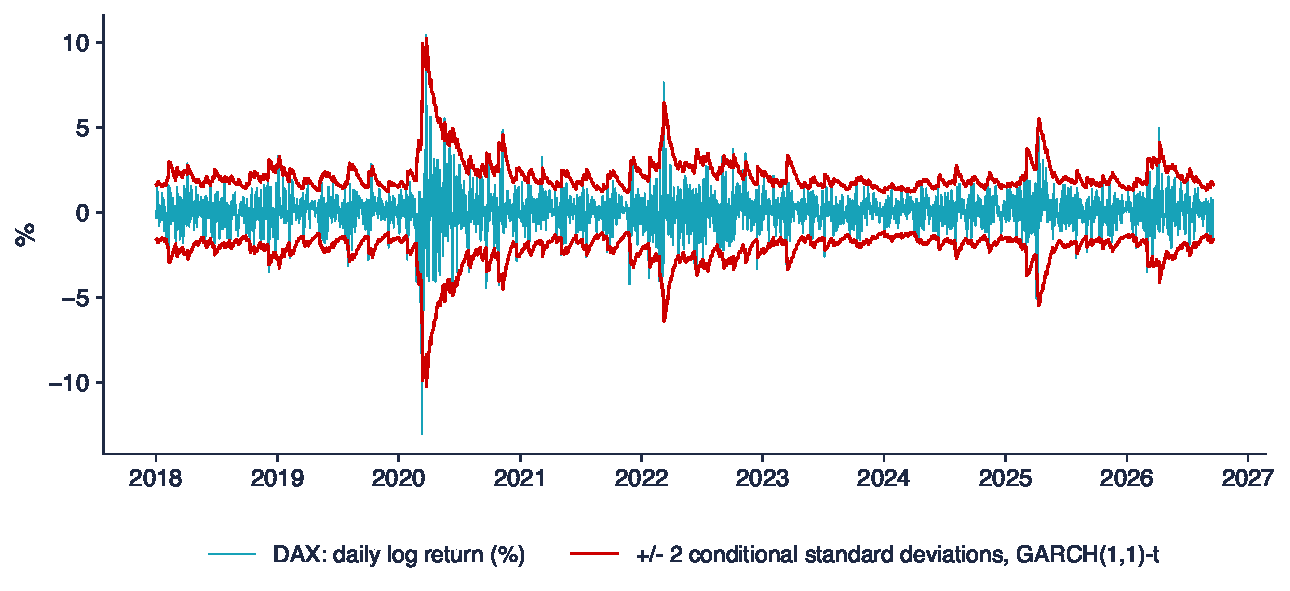
\includegraphics[width=0.96\textwidth,height=0.30\textheight,keepaspectratio]{ch9_sem_b1.pdf}
\end{center}
\vspace{-2mm}
\begin{center}
\scriptsize
\begin{tabular}{lrrrrr}
\toprule
& $\mu$ & $\omega$ & $\alpha$ & $\beta$ & $\nu$ \\
\midrule
estimate & $0.081$ & $0.0206$ & $0.097$ & $0.895$ & $7.08$ \\
robust SE & $0.012$ & $0.0049$ & $0.011$ & $0.012$ & $0.62$ \\
\bottomrule
\end{tabular}
\end{center}
\begin{itemize}
    \item $T = 6\,786$; $\alpha + \beta = 0.992$, half-life $\ln 0.5/(-0.00784) = 88.5$ days; long-run volatility 25.9\% against 22.4\% in the sample
    \item Peaks: 80\% (2008), 82\% (2020); last day: 13.0\%; 5.2\% of the days fall outside $\pm 2\hat\sigma_t$
    \item Interpretation: the current one: VaR for tomorrow needs $\sigma_{t+1}$; the long-run level matters only for long horizons, and it is imprecise because $1 - \alpha - \beta = 0.0078$ is small
\end{itemize}\sfmquantlet{Ch_09}{SFM_ch9_seminar}
\end{frame}

\begin{frame}{B2: BET, Banca Transilvania and Bitcoin [Proposed]}
\itemsize{\footnotesize}
\begin{itemize}
\item \textbf{Question}: which of the BET, Banca Transilvania and Bitcoin has the most persistent volatility? Model: B1.
\item \textbf{Inputs}: BET since 2000, TLV since 2010 (without 30--31 May 2016), Bitcoin since 2014; daily log returns in \%
\item \textbf{Tasks}
\begin{enumerate}
    \item Estimate GARCH(1,1)-t for each series and report $\alpha$, $\beta$ and $\nu$.
    \item Compute the persistence, the half-life and the long-run volatility where they exist.
    \item Compare the long-run with the sample volatility (annualise Bitcoin with 365 days).
    \item Interpretation: what does an estimate $\hat\alpha + \hat\beta = 1$ tell a risk manager?
\end{enumerate}
\item \textbf{Report}: one table and two sentences
\item Notebook: section B2
\end{itemize}
\end{frame}

\ifsolutions
\begin{frame}{B2: Solution [Proposed]}
\itemsize{\footnotesize}
\begin{center}
\scriptsize
\begin{tabular}{lrrrrrrrrr}
\toprule
& $T$ & $\alpha$ & $\beta$ & $\nu$ & $\alpha + \beta$ & half-life & long-run vol. & sample vol. & peak 2020 \\
\midrule
BET & 6\,670 & $0.192$ & $0.799$ & $5.01$ & $0.991$ & 74.3 & 34.7 & 22.1 & 88 \\
TLV & 3\,788 & $0.139$ & $0.824$ & $4.91$ & $0.963$ & 18.4 & 28.2 & 26.5 & 80 \\
Bitcoin & 4\,384 & $0.109$ & $0.891$ & $3.18$ & $1.000$ & -- & -- & 66.6 & 301 \\
\bottomrule
\end{tabular}
\end{center}
\begin{itemize}
    \item BET: the strongest reaction ($\alpha = 0.192$) and a half-life of 74.3 days; its long-run volatility (34.7\%) is far above the sample value: an imprecise number
    \item TLV: shorter memory (18.4 days); long-run and sample volatility agree (28.2\% and 26.5\%)
    \item Bitcoin: $\hat\alpha + \hat\beta = 1.0000$: an IGARCH, the most persistent; $\hat\nu = 3.18$
    \item Interpretation: no mean reversion: forecasts for every horizon equal today's variance; the model behaves like an EWMA, and a long-run volatility should not be reported
\end{itemize}\sfmquantlet{Ch_09}{SFM_ch9_seminar}
\end{frame}
\fi

\begin{frame}{B3: The Leverage Effect in the S\&P 500 [Solved]}
\itemsize{\footnotesize}
\begin{itemize}
\item \textbf{Question}: do falls raise the volatility of the S\&P 500 more than rises of the same size?
\item \textbf{Inputs}: S\&P 500 closes since 2000, daily log returns in \%
\item \textbf{Tasks}
\begin{enumerate}
    \item Estimate GARCH(1,1)-t and GJR-GARCH(1,1)-t; report $\gamma$ with its robust $t$ statistic.
    \item Compute the LR statistic of GJR against GARCH, its p-value and the two BIC values.
    \item Run the sign-bias test on the standardised residuals of GARCH-t.
    \item Draw both news impact curves and compute the GJR variance after shocks of $-2\%$ and $+2\%$.
    \item Interpretation: how does the leverage effect change the VaR on the day after a fall?
\end{enumerate}
\item \textbf{Report}: four statistics with p-values, two variances, the chart and two sentences
\item Notebook: section B3
\end{itemize}
\end{frame}

\begin{frame}{B3: Solution [Solved]}
\itemsize{\scriptsize}
\begin{center}
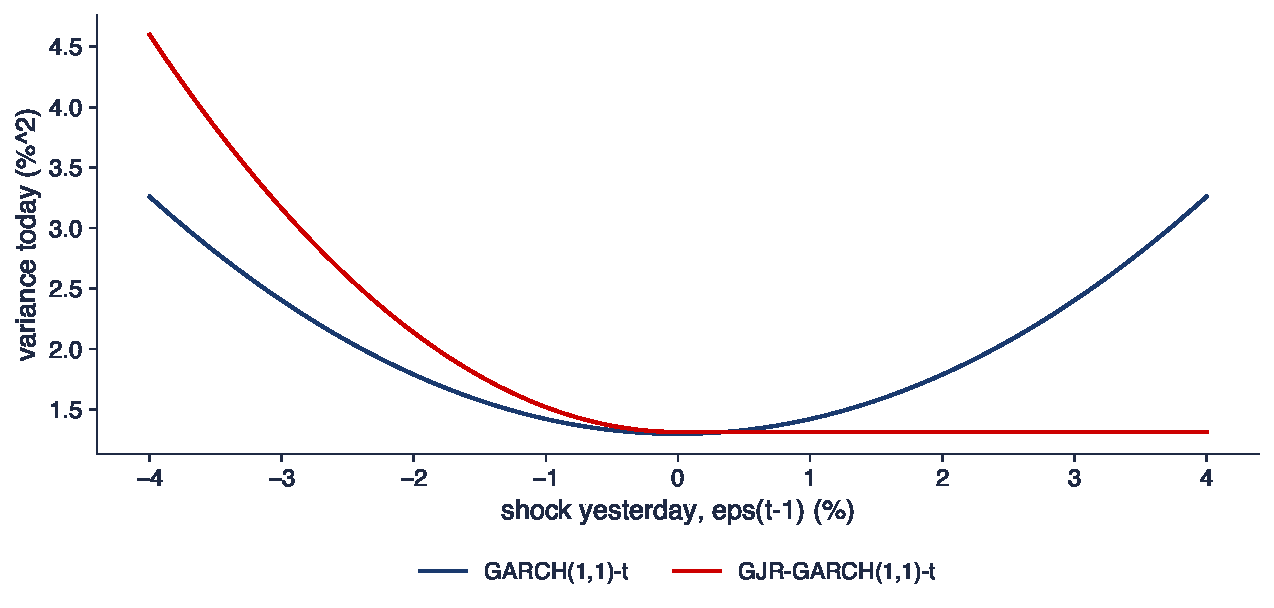
\includegraphics[width=0.96\textwidth,height=0.34\textheight,keepaspectratio]{ch9_sem_b3.pdf}
\end{center}
\vspace{-2mm}
\begin{itemize}
    \item GJR: $\hat\alpha = 0.000$, $\hat\gamma = 0.205$ ($t = 10.03$), $\hat\beta = 0.881$; LR $= 235.7$ (p $<$\,0.001); BIC $18169.0 \to 17942.2$
    \item Sign bias on GARCH-t residuals: $\chi^2(3) = 40.7$ (p $<$\,0.001), sign $t = 3.56$
    \item GJR variance after $-2\%$: $2.136$; after $+2\%$: $1.315$; ratio $1.62$
    \item Interpretation: only falls raise the variance ($\hat\alpha = 0$); after a fall the VaR is about $\sqrt{1.62}$ times the VaR after an equal rise; a symmetric GARCH understates risk after bad days
\end{itemize}\sfmquantlet{Ch_09}{SFM_ch9_seminar}
\end{frame}

\begin{frame}{B4: Asymmetry on the BVB and in Bitcoin [Proposed]}
\itemsize{\footnotesize}
\begin{itemize}
\item \textbf{Question}: is there a leverage effect in the BET, in Banca Transilvania and in Bitcoin? Model: B3.
\item \textbf{Inputs}: BET since 2000, TLV since 2010, Bitcoin since 2014; daily log returns in \%
\item \textbf{Tasks}
\begin{enumerate}
    \item Estimate GJR-GARCH(1,1)-t and EGARCH(1,1)-t; report both $\gamma$ with robust $t$ statistics.
    \item Compute the LR test of GJR against GARCH and the change in BIC.
    \item Compute the GJR ratio of the variances after $-2\%$ and $+2\%$.
    \item Interpretation: would you use an asymmetric model for each of the three? Why?
\end{enumerate}
\item \textbf{Report}: one table and two sentences
\item Notebook: section B4
\end{itemize}
\end{frame}

\ifsolutions
\begin{frame}{B4: Solution [Proposed]}
\itemsize{\footnotesize}
\begin{center}
\footnotesize
\begin{tabular}{lrrrrrrrr}
\toprule
& GJR $\gamma$ & $t$ & LR & p & $\Delta$BIC & EGARCH $\gamma$ & $t$ & ratio $-2/+2$ \\
\midrule
BET & $0.043$ & ${2.05}$ & $4.9$ & 0.026 & ${3.9}$ & ${-0.028}$ & ${-2.63}$ & $1.08$ \\
TLV & $0.065$ & ${2.71}$ & $7.8$ & 0.005 & ${0.4}$ & ${-0.040}$ & ${-3.00}$ & $1.08$ \\
Bitcoin & $-0.013$ & ${-0.72}$ & $0.7$ & 0.416 & ${7.7}$ & ${0.015}$ & ${1.18}$ & $1.00$ \\
\bottomrule
\end{tabular}
\end{center}
\begin{itemize}
    \item BET and TLV: $\gamma > 0$ (EGARCH $\gamma < 0$), significant by LR at 5\%, but BIC rises ($\Delta$BIC $> 0$) and the ratio is only 1.08 and 1.08
    \item Bitcoin: no asymmetry at all ($t = -0.72$; ratio 1.00)
    \item Interpretation: for the BVB the effect is real but small: GARCH-t is enough for most uses; for Bitcoin a symmetric model is right; for the S\&P 500 (B3) asymmetry is essential
\end{itemize}\sfmquantlet{Ch_09}{SFM_ch9_seminar}
\end{frame}
\fi

\begin{frame}{B5: GARCH against EWMA for the S\&P 500 [Solved]}
\itemsize{\footnotesize}
\begin{itemize}
\item \textbf{Question}: does GARCH(1,1)-t forecast tomorrow's variance of the S\&P 500 better than EWMA, and is its VaR 1\% exceeded on 1\% of days?
\item \textbf{Inputs}: S\&P 500 since 2000; forecasts for every day since 2 January 2015
\item \textbf{Tasks}
\begin{enumerate}
    \item Re-estimate GARCH(1,1)-t every 250 days on all data up to that day and compute the one-day forecasts $h_t$; compute EWMA with $\lambda = 0.94$.
    \item Compute the mean QLIKE of both models and the Diebold--Mariano $t$ statistic.
    \item Count the exceedances of the GARCH-t VaR 1\% and of the EWMA-Normal VaR 1\% and compare with the expected number.
    \item Draw the cumulative difference of the losses.
    \item Interpretation: which model would you give to a risk manager, and what would you still fix?
\end{enumerate}
\item \textbf{Report}: four numbers, two counts, the chart and two sentences
\item Notebook: section B5
\end{itemize}
\end{frame}

\begin{frame}{B5: Solution [Solved]}
\itemsize{\scriptsize}
\begin{center}
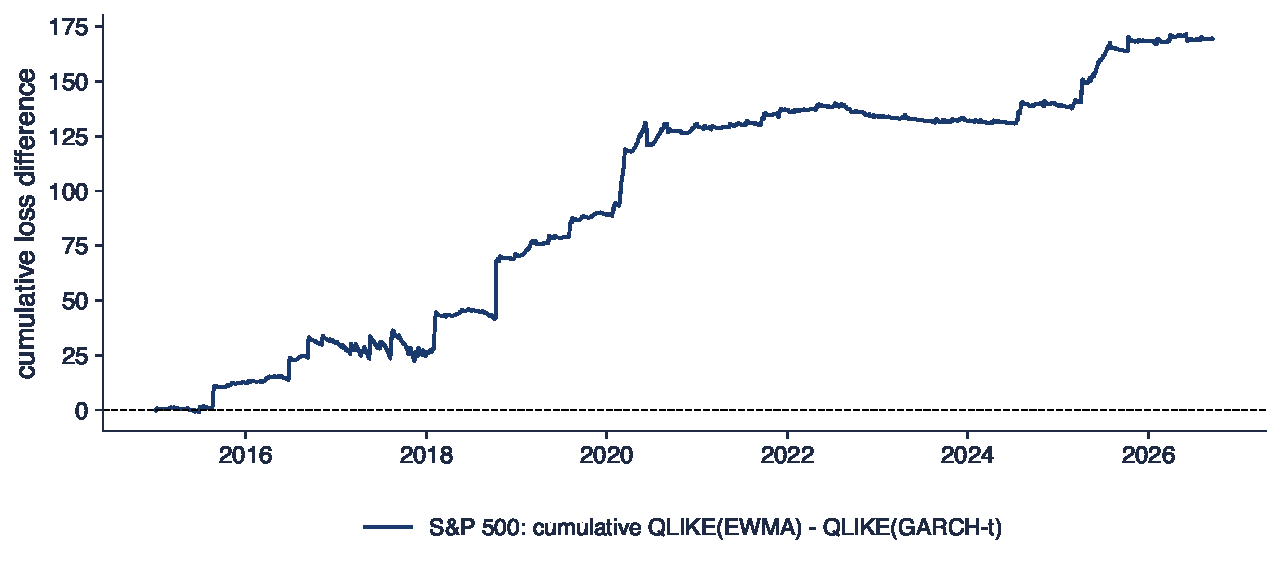
\includegraphics[width=0.96\textwidth,height=0.32\textheight,keepaspectratio]{ch9_sem_b5.pdf}
\end{center}
\vspace{-2mm}
\begin{itemize}
    \item 2\,944 days; mean QLIKE: GARCH-t $0.761$, EWMA $0.819$; DM: mean difference $-0.058$, $t = -3.69$ (p $<$\,0.001): GARCH-t is better
    \item VaR 1\% exceedances: GARCH-t 49 (1.66\%), EWMA-Normal 65 (2.21\%); expected about 29
    \item Interpretation: GARCH-t, but both VaR models are exceeded too often; add the leverage effect (B3) and test the exceedances formally (Chapter 10)
\end{itemize}\sfmquantlet{Ch_09}{SFM_ch9_seminar}
\end{frame}

\begin{frame}{B6: GARCH against EWMA for the DAX and the BET [Proposed]}
\itemsize{\footnotesize}
\begin{itemize}
\item \textbf{Question}: does the result of B5 hold for the DAX and for the BET? Model: B5.
\item \textbf{Inputs}: DAX and BET since 2000; forecasts for every day since January 2015
\item \textbf{Tasks}
\begin{enumerate}
    \item Compute the out-of-sample GARCH(1,1)-t and EWMA forecasts as in B5.
    \item Compute the mean QLIKE of both models and the DM test.
    \item Count the VaR 1\% exceedances of both models.
    \item Interpretation: for which index does GARCH help most, and why?
\end{enumerate}
\item \textbf{Report}: one table and two sentences
\item Notebook: section B6
\end{itemize}
\end{frame}

\ifsolutions
\begin{frame}{B6: Solution [Proposed]}
\itemsize{\footnotesize}
\begin{center}
\scriptsize
\begin{tabular}{lrrrrrrr}
\toprule
& days & QLIKE GARCH-t & QLIKE EWMA & DM $t$ (p) & expected & exc. GARCH-t & exc. EWMA \\
\midrule
DAX & 2\,973 & $1.090$ & $1.121$ & ${-3.19}$ (0.001) & 30 & 45 (1.51\%) & 74 (2.49\%) \\
BET & 2\,926 & $0.680$ & $0.788$ & ${-2.22}$ (0.027) & 29 & 34 (1.16\%) & 67 (2.29\%) \\
\bottomrule
\end{tabular}
\end{center}
\begin{itemize}
    \item Both indices: GARCH-t has the smaller QLIKE, significant at 5\% by DM
    \item BET: the largest QLIKE gain and an almost exact VaR (1.16\% against 1\%); EWMA-Normal is exceeded about twice as often as it should be
    \item Interpretation: the BET has heavy tails ($\nu \approx 5$) and sudden jumps of volatility: the Student-t quantile and the mean reversion of GARCH both help
\end{itemize}\sfmquantlet{Ch_09}{SFM_ch9_seminar}
\end{frame}
\fi


%=============================================================================
\section{Part C: Open Questions and AI Critique}
%=============================================================================

\begin{frame}{C1: Is Bitcoin Volatility Becoming Equity-Like? [Proposed]}
\itemsize{\footnotesize}
\begin{itemize}
\item \textbf{Question}: has Bitcoin volatility moved closer to the volatility of the S\&P 500 since 2021?
\item \textbf{Inputs}: Bitcoin and S\&P 500 daily log returns, 2015--2019 and 2021--2026; models: B1, B3
\item \textbf{Tasks}
\begin{enumerate}
    \item Estimate GJR-GARCH(1,1)-t for both series in both periods and report the persistence, $\gamma$ and $\nu$.
    \item Compute the correlation of the logarithms of the two GARCH-t volatilities on common days in each period.
    \item List the events of 2020--2024 that could explain a change.
    \item Interpretation: how would you separate a lasting change from a change caused by one crisis?
\end{enumerate}
\item \textbf{Report}: a table and a plan for a project
\item Notebook: section C1
\end{itemize}
\end{frame}

\ifsolutions
\begin{frame}{C1: Reference Analysis [Proposed]}
\itemsize{\footnotesize}
\begin{center}
\scriptsize
\begin{tabular}{lrrrrrr}
\toprule
Period & BTC $\alpha + \beta + \gamma/2$ & BTC $\gamma$ ($t$) & BTC $\nu$ & S\&P persistence & S\&P $\gamma$ ($t$) & corr.\ of log-vol. \\
\midrule
2015--2019 & 1.000 & $-0.059$ ($-2.5$) & $3.23$ & $0.968$ & $0.344$ ($5.0$) & $0.04$ \\
2021--2026 & 1.000 & $0.037$ ($1.4$) & $3.28$ & $0.971$ & $0.196$ ($4.1$) & $0.32$ \\
\bottomrule
\end{tabular}
\end{center}
\begin{itemize}
    \item Bitcoin 2015--2019: $\gamma = -0.059$ ($t = -2.5$): rises raised volatility more than falls (an inverse leverage effect); 2021--2026: $\gamma = 0.037$ ($t = 1.4$), not significant
    \item Correlation of the two volatilities: from $0.04$ to $0.32$; sample volatility of Bitcoin: from 74.3\% to 57.1\%; still IGARCH-like
    \item Events: COVID-19 (2020), institutional buying (2021), the crypto crash of 2022, spot Bitcoin ETFs (2024); design: rolling windows, Ethereum and gold as controls, a test of the change in the correlation
\end{itemize}\sfmquantlet{Ch_09}{SFM_ch9_seminar}
\end{frame}
\fi

\begin{frame}{C2: Audit an AI Answer [Proposed]}
\itemsize{\scriptsize}
\begin{itemize}
    \item A student asked an AI assistant to interpret a GARCH(1,1)-t fit of the S\&P 500 (daily, since 2000): $\hat\omega = 0.0157$, $\hat\alpha = 0.123$, $\hat\beta = 0.872$, $\hat\nu = 6.26$. The answer:
    \item \aiprompt{(a) alpha + beta = 0.995, so a volatility shock disappears within about a week.}
    \item \aiprompt{(b) The long-run variance is omega/(1 - alpha) = 0.018, an annual volatility of 2.1\%.}
    \item \aiprompt{(c) A GJR fit gives gamma = 0.205 > 0: good news raises volatility more than bad news.}
    \item \aiprompt{(d) Ljung-Box Q(10) of the squared standardised residuals = 13.6, p = 0.19: the GARCH-t model is correct.}
    \item \aiprompt{(e) With Student-t innovations the one-day VaR 1\% is 2.326 times sigma(t+1).}
    \item \aiprompt{(f) EWMA with lambda = 0.94 is a GARCH(1,1) with omega = 0, alpha = 0.06, beta = 0.94.}
    \item Tasks
    \begin{itemize}
        \item 1. For each statement, say whether it is correct; if not, give the correct statement and, where possible, the correct number from the notebook (section C2).
        \item 2. Report: a list of six verdicts with one line of justification each.
    \end{itemize}
\end{itemize}
\end{frame}

\ifsolutions
\begin{frame}{C2: Solution [Proposed]}
\itemsize{\footnotesize}
\begin{itemize}
    \item (a) Wrong: the half-life is $\ln 0.5/\ln 0.995 = 131$ days, about half a year
    \item (b) Wrong: $\bar\sigma^2 = \omega/(1 - \alpha - \beta) = 2.97$, a long-run volatility of 27.3\% (imprecise, since $1 - \alpha - \beta$ is small)
    \item (c) Wrong: $\gamma > 0$ adds to the slope of \textbf{negative} shocks: bad news raises volatility more (the leverage effect)
    \item (d) Wrong: no ARCH effect is left, but this does not prove the model correct; the sign-bias test rejects ($\chi^2(3) = 40.7$): the asymmetry is missing
    \item (e) Wrong: 2.326 is the Normal quantile; for the standardised $t$ with $\nu = 6.26$ the factor is $2.557$
    \item (f) Correct: EWMA is an IGARCH without a constant
\end{itemize}\sfmquantlet{Ch_09}{SFM_ch9_seminar}
\end{frame}
\fi


%=============================================================================
\section{Wrap-Up}
%=============================================================================

\begin{frame}{What You Should Take from Today}
\itemsize{\small}
\begin{itemize}
    \item $\alpha + \beta$ decides everything long-run: half-life, long-run variance, the shape of the forecasts
    \item Multi-day risk is the sum of the daily variance forecasts, not $\sqrt{H}$ times today's volatility
    \item Heavy-tailed innovations change the VaR quantile; asymmetry changes the VaR after bad days
    \item Compare forecasts out of sample (QLIKE, DM), not only in sample (AIC, BIC)
    \item An AI answer is a draft: check the formula of the long-run variance, the sign of $\gamma$ and the quantile
\end{itemize}
\end{frame}

\begin{frame}{After the Seminar}
\itemsize{\small}
\begin{itemize}
    \item Lecture 9 develops each topic of today: ARCH and GARCH, estimation, innovations, asymmetry, diagnostics, forecasts, VaR
    \item Try the [Proposed] tasks in the notebook; the solutions are discussed in class
    \item C1 can grow into a team project: rolling windows, Ethereum and gold as controls
    \item Reading: \refFHH, Ch.~13; exercises in \refBHL, Ch.~13; \refTsay, Ch.~3
\end{itemize}
\end{frame}


%=============================================================================
\section{References}
%=============================================================================

\begin{frame}{References}
\itemsize{\tiny}
\begin{itemize}
    \item Bollerslev, T. (1986). \href{https://doi.org/10.1016/0304-4076(86)90063-1}{Generalized autoregressive conditional heteroskedasticity}. \textit{Journal of Econometrics}, 31(3), 307--327.
    \item Bollerslev, T. (1987). \href{https://doi.org/10.2307/1925546}{A conditionally heteroskedastic time series model for speculative prices and rates of return}. \textit{Review of Economics and Statistics}, 69(3), 542--547.
    \item Bollerslev, T., Wooldridge, J.M. (1992). \href{https://doi.org/10.1080/07474939208800229}{Quasi-maximum likelihood estimation and inference in dynamic models with time-varying covariances}. \textit{Econometric Reviews}, 11(2), 143--172.
    \item Borak, S., Härdle, W.K., López-Cabrera, B. (2013). \href{https://doi.org/10.1007/978-3-642-33929-5}{\textit{Statistics of Financial Markets: Exercises and Solutions}}, 2nd ed. Springer.
    \item Christie, A.A. (1982). \href{https://doi.org/10.1016/0304-405X(82)90018-6}{The stochastic behavior of common stock variances: value, leverage and interest rate effects}. \textit{Journal of Financial Economics}, 10(4), 407--432.
    \item Diebold, F.X., Mariano, R.S. (1995). \href{https://doi.org/10.1080/07350015.1995.10524599}{Comparing predictive accuracy}. \textit{Journal of Business \& Economic Statistics}, 13(3), 253--263.
    \item Engle, R.F. (1982). \href{https://doi.org/10.2307/1912773}{Autoregressive conditional heteroscedasticity with estimates of the variance of United Kingdom inflation}. \textit{Econometrica}, 50(4), 987--1007.
    \item Engle, R.F., Ng, V.K. (1993). \href{https://doi.org/10.1111/j.1540-6261.1993.tb05127.x}{Measuring and testing the impact of news on volatility}. \textit{Journal of Finance}, 48(5), 1749--1778.
    \item Franke, J., Härdle, W.K., Hafner, C.M. (2019). \href{https://doi.org/10.1007/978-3-030-13751-9}{\textit{Statistics of Financial Markets: An Introduction}}, 5th ed. Springer.
    \item Glosten, L.R., Jagannathan, R., Runkle, D.E. (1993). \href{https://doi.org/10.1111/j.1540-6261.1993.tb05128.x}{On the relation between the expected value and the volatility of the nominal excess return on stocks}. \textit{Journal of Finance}, 48(5), 1779--1801.
    \item Hansen, B.E. (1994). \href{https://doi.org/10.2307/2527081}{Autoregressive conditional density estimation}. \textit{International Economic Review}, 35(3), 705--730.
    \item Ljung, G.M., Box, G.E.P. (1978). \href{https://doi.org/10.1093/biomet/65.2.297}{On a measure of lack of fit in time series models}. \textit{Biometrika}, 65(2), 297--303.
    \item Nelson, D.B. (1991). \href{https://doi.org/10.2307/2938260}{Conditional heteroskedasticity in asset returns: a new approach}. \textit{Econometrica}, 59(2), 347--370.
    \item Patton, A.J. (2011). \href{https://doi.org/10.1016/j.jeconom.2010.03.034}{Volatility forecast comparison using imperfect volatility proxies}. \textit{Journal of Econometrics}, 160(1), 246--256.
    \item Tsay, R.S. (2010). \href{https://doi.org/10.1002/9780470644560}{\textit{Analysis of Financial Time Series}}, 3rd ed. Wiley.
\end{itemize}
\end{frame}

\end{document}
